\chapter{Studiu Bibliografic}\label{ch:studiubib}
\pagestyle{fancy}
%%%%%%%%%%%%%%%%%%%%%%%%%%%%%%%%%%%%%%%%%%%%%%%%%%%%%%%%%%%%%%%%%%%%%%%%%%%%%%%%%%%%%%%%%%%%%%%%%%%%%%%%%%%%%%%%%%%%%%%%%%%%%%%%%%%%%%%%%%%%
\section{Modul backend}
\subsection{Arhitectura Client-Server}
Acest tip de arhitectură este folosită pentru a separa sarcinile între client și server. Folosind un mecanism de tip request-reponse, procesul este următorul:
\vspace{0.5mm}
\begin{itemize}
	\setlength\itemsep{0.5em}
    \item Clientul face un request la server pentru a obține o anumită resursă
    \item Serverul trimite un răspuns per request clientului
    \item Conexiunea poate fi închisă de oricare dintre cei doi
\end{itemize}

\ \\
\begin{figure}[ht]
	\centering
	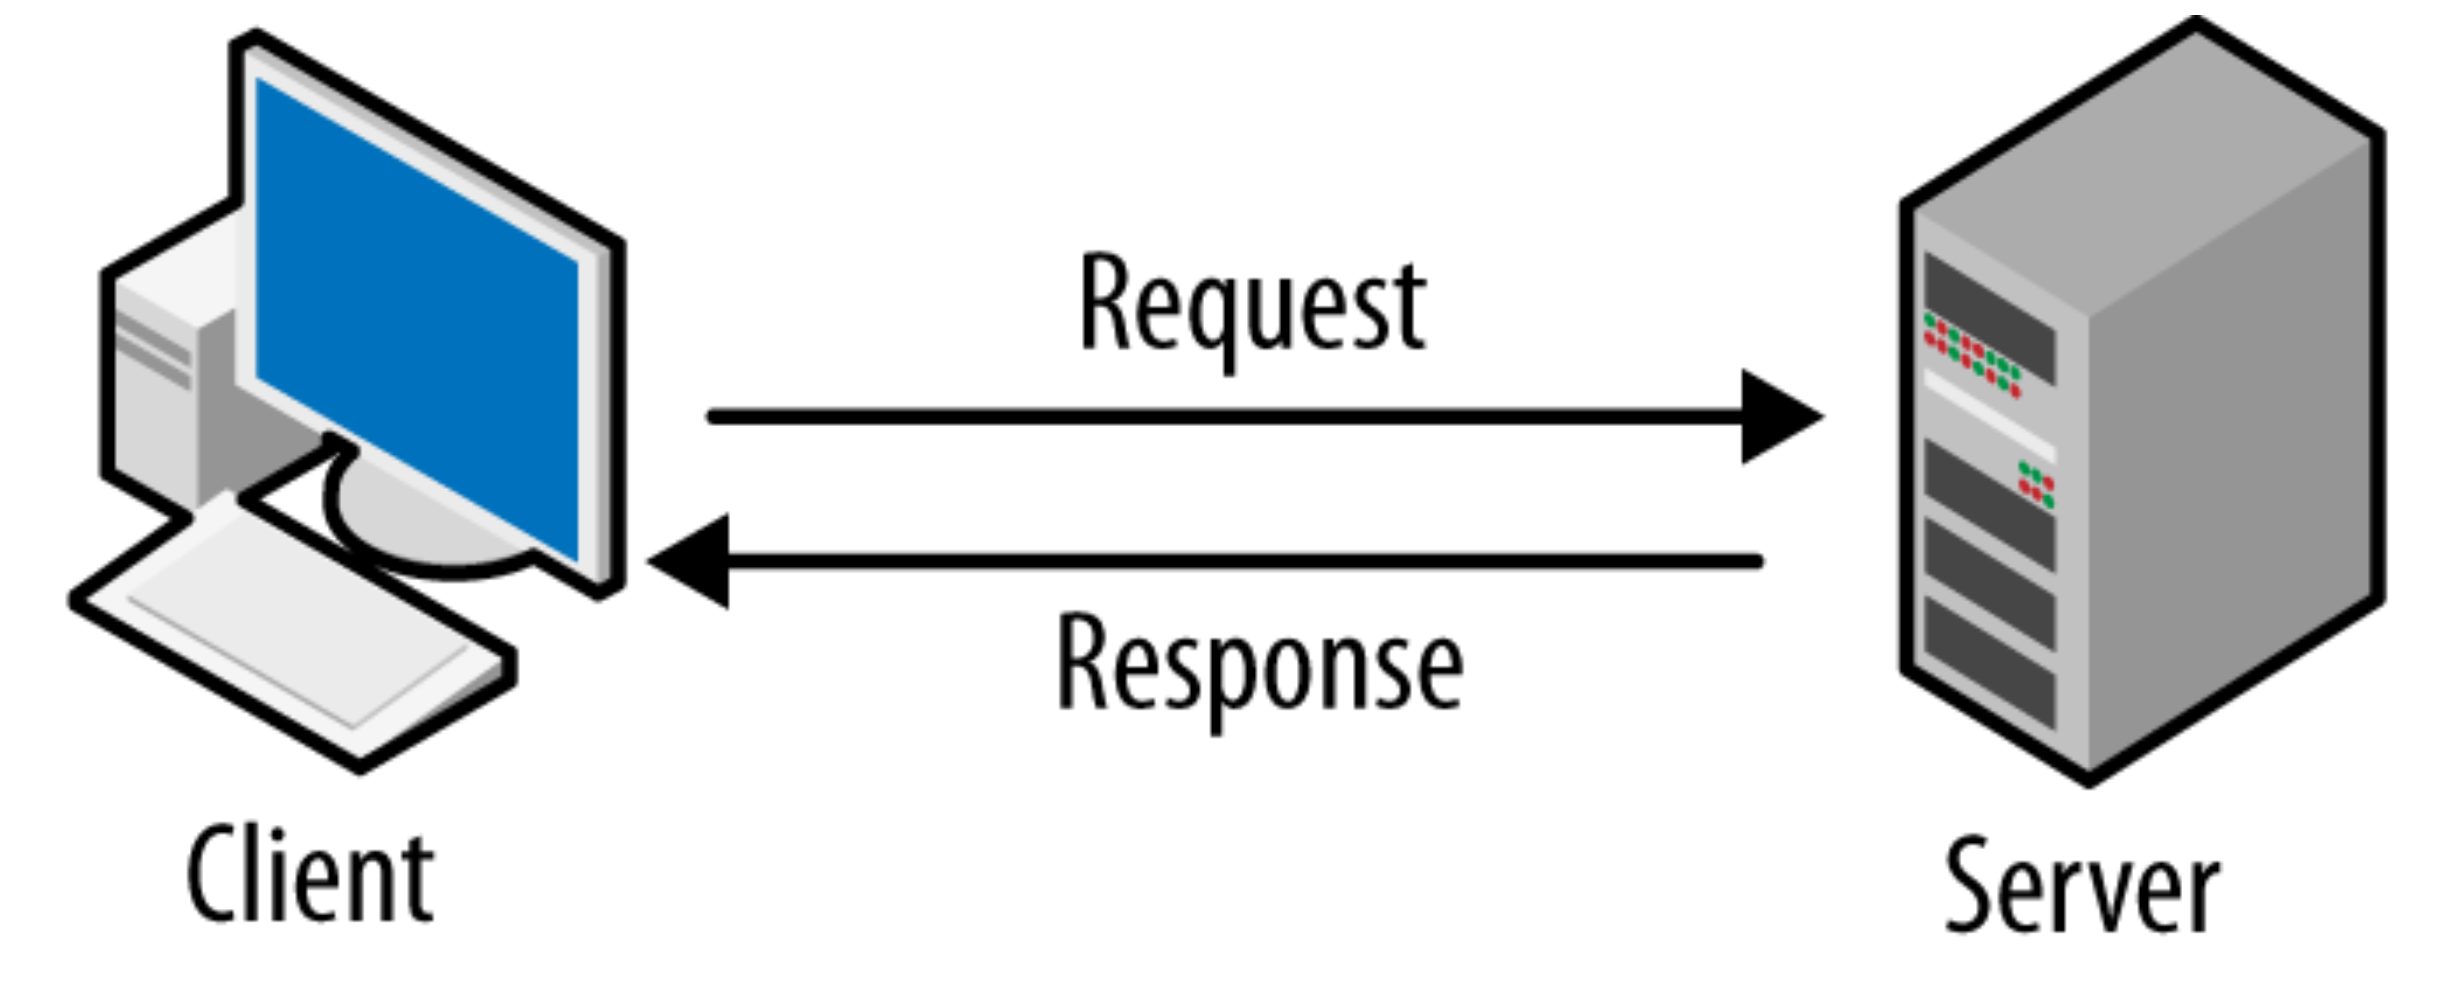
\includegraphics[width=100mm, scale=2]{figs/clientServerArch.png}
    \caption{Arhitectura 3-tier. Sursa~\cite{ClientServer}}
	\label{fig:clientServerArch}
\end{figure}
\ \\

Protocolul HTTP este un protocol request-reponse, care se bazează pe o arhitectură client-server. \\

Un {\it HTTP request} reprezintă modalitatea prin care browserul web, în cazul acestui proiect, solicită resurse. Fiecare request conține:
\begin{itemize}
	\setlength\itemsep{0.5em}
    \item Versiunea HTTP
    \item URL (Uniform Resource Locator)
    \begin{itemize}
		\setlength\itemsep{0.5em}
        \item Informații despre locația resursei solicitată de client
    \end{itemize}
    \item Metoda HTTP
    \begin{itemize}
		\setlength\itemsep{0.5em}
        \begingroup \color{blue}
        \item GET \endgroup
        \item HEAD
        \begingroup \color{blue}
        \item POST \endgroup
        \begingroup \color{blue}
        \item GET \endgroup
        \begingroup \color{blue}
        \item DELETE \endgroup
        \item TRACE
        \item OPTIONS
        \item CONNECT
        \item PATCH
    \end{itemize}
    \item HTTP Request Header
    \begin{itemize}
		\setlength\itemsep{0.5em}
        \item Conține informații despre browser-ul clientului, resursa cerută, encoding, server, etc.
    \end{itemize}
    \item Body (opțional, doar pentru anumite requesturi)
    \begin{itemize}
		\setlength\itemsep{0.5em}
        \item Conține informații transmise serverului (pentru anumite metode HTTP)
    \end{itemize}
\end{itemize}
\ \\

Un {\it HTTP response} este informația pe care o primesc clienții de la server ca răspuns la request. Acest răspuns conține:
\begin{itemize}
	\setlength\itemsep{0.5em}
    \item Status
    \begin{itemize}
		\setlength\itemsep{0.5em}
        \item Cod din 3 cifre care indică dacă requestul a fost încheiat cu succes
    \end{itemize}
    \item HTTP Response Header
    \begin{itemize}
		\setlength\itemsep{0.5em}
        \item Conține informații despre limba și formatul conținutului din body
    \end{itemize}
    \item Body
    \begin{itemize}
		\setlength\itemsep{0.5em}
        \item Conține informația solicitată printr-un request
    \end{itemize}
\end{itemize}
%%%%%%%%%%%%%%%%%%%%%%%%%%%%%%%%%%%%%%%%%%%%%%%%%%%%%%%%%%%%%%%%%%%%%%%%%%%%%%%%%%%%%%%%%%%%%%%%%%%%%%%%%%%%%%%%%%%%%%%%%%%%%%%%%%%%%%%%%%%%
\subsection{Arhitectura 3-Tier}
Arhitectura 3-Tier sau 3-Layer este o arhitectură pe 3 nivele: 
\begin{itemize}
	\setlength\itemsep{0.5em}
    \item Nivelul prezentării
    \begin{itemize}
        \setlength\itemsep{0.5em}
        \item Acest nivel este reprezentat de modulul de front-end al aplicație, interfața cu care utilizatorii vor interacționa în mod direct
        \item Acest nivel a fost construit în aplicație folosind:
        \begin{itemize}
            \setlength\itemsep{0.5em}
            \item Librăria {\it React Typescript}
            \item Pentru componente, este utilizată libraria {\it Ant Design}
            \item Pentru customizarea componentelor s-a utilizat {\it Styled Components}, un framework pentru stilizare, CSS-in-JS
        \end{itemize}
    \end{itemize}
    \item Nivelul aplicației
    \begin{itemize}
        \setlength\itemsep{0.5em}
        \item Acest nivel este reprezentat de modulul de back-end al aplicației
        \item Aici sunt procesate informațiile primite de la nivelul superior, cel de prezentare
        \item Nivelul interacționează în mod direct cu serverul. Acesta transmite cererea clientului la server, la fel și răspunsul serverului către client
        \item Pentru implementarea acestui nivel în aplicație, am folosit:
        \begin{itemize}
            \setlength\itemsep{0.5em}
            \item .NET Framework
            \item Entity Framework Core, un Object-Relational Mapper, care creează un layer între limbaj și baza de date
            \item MediatR, implementarea în .NET a patternului
        \end{itemize}
    \end{itemize}
    \item Nivelul datelor
    \begin{itemize}
        \setlength\itemsep{0.5em}
        \item Cunoscut ca nivelul bazei de date
        \item Aici se găsesc servere de baze de date unde se pot stoca și prelua informații
        \item Pentru acest nivel, am folosit Microsoft SQL Server
    \end{itemize}
\end{itemize}
\vspace{1em}
Avantajul utilizării acestui pattern arhitectural este că permite ca un layer să fie modificat, fără să fie afectate celelalte.
\begin{figure}[h]
	\centering
	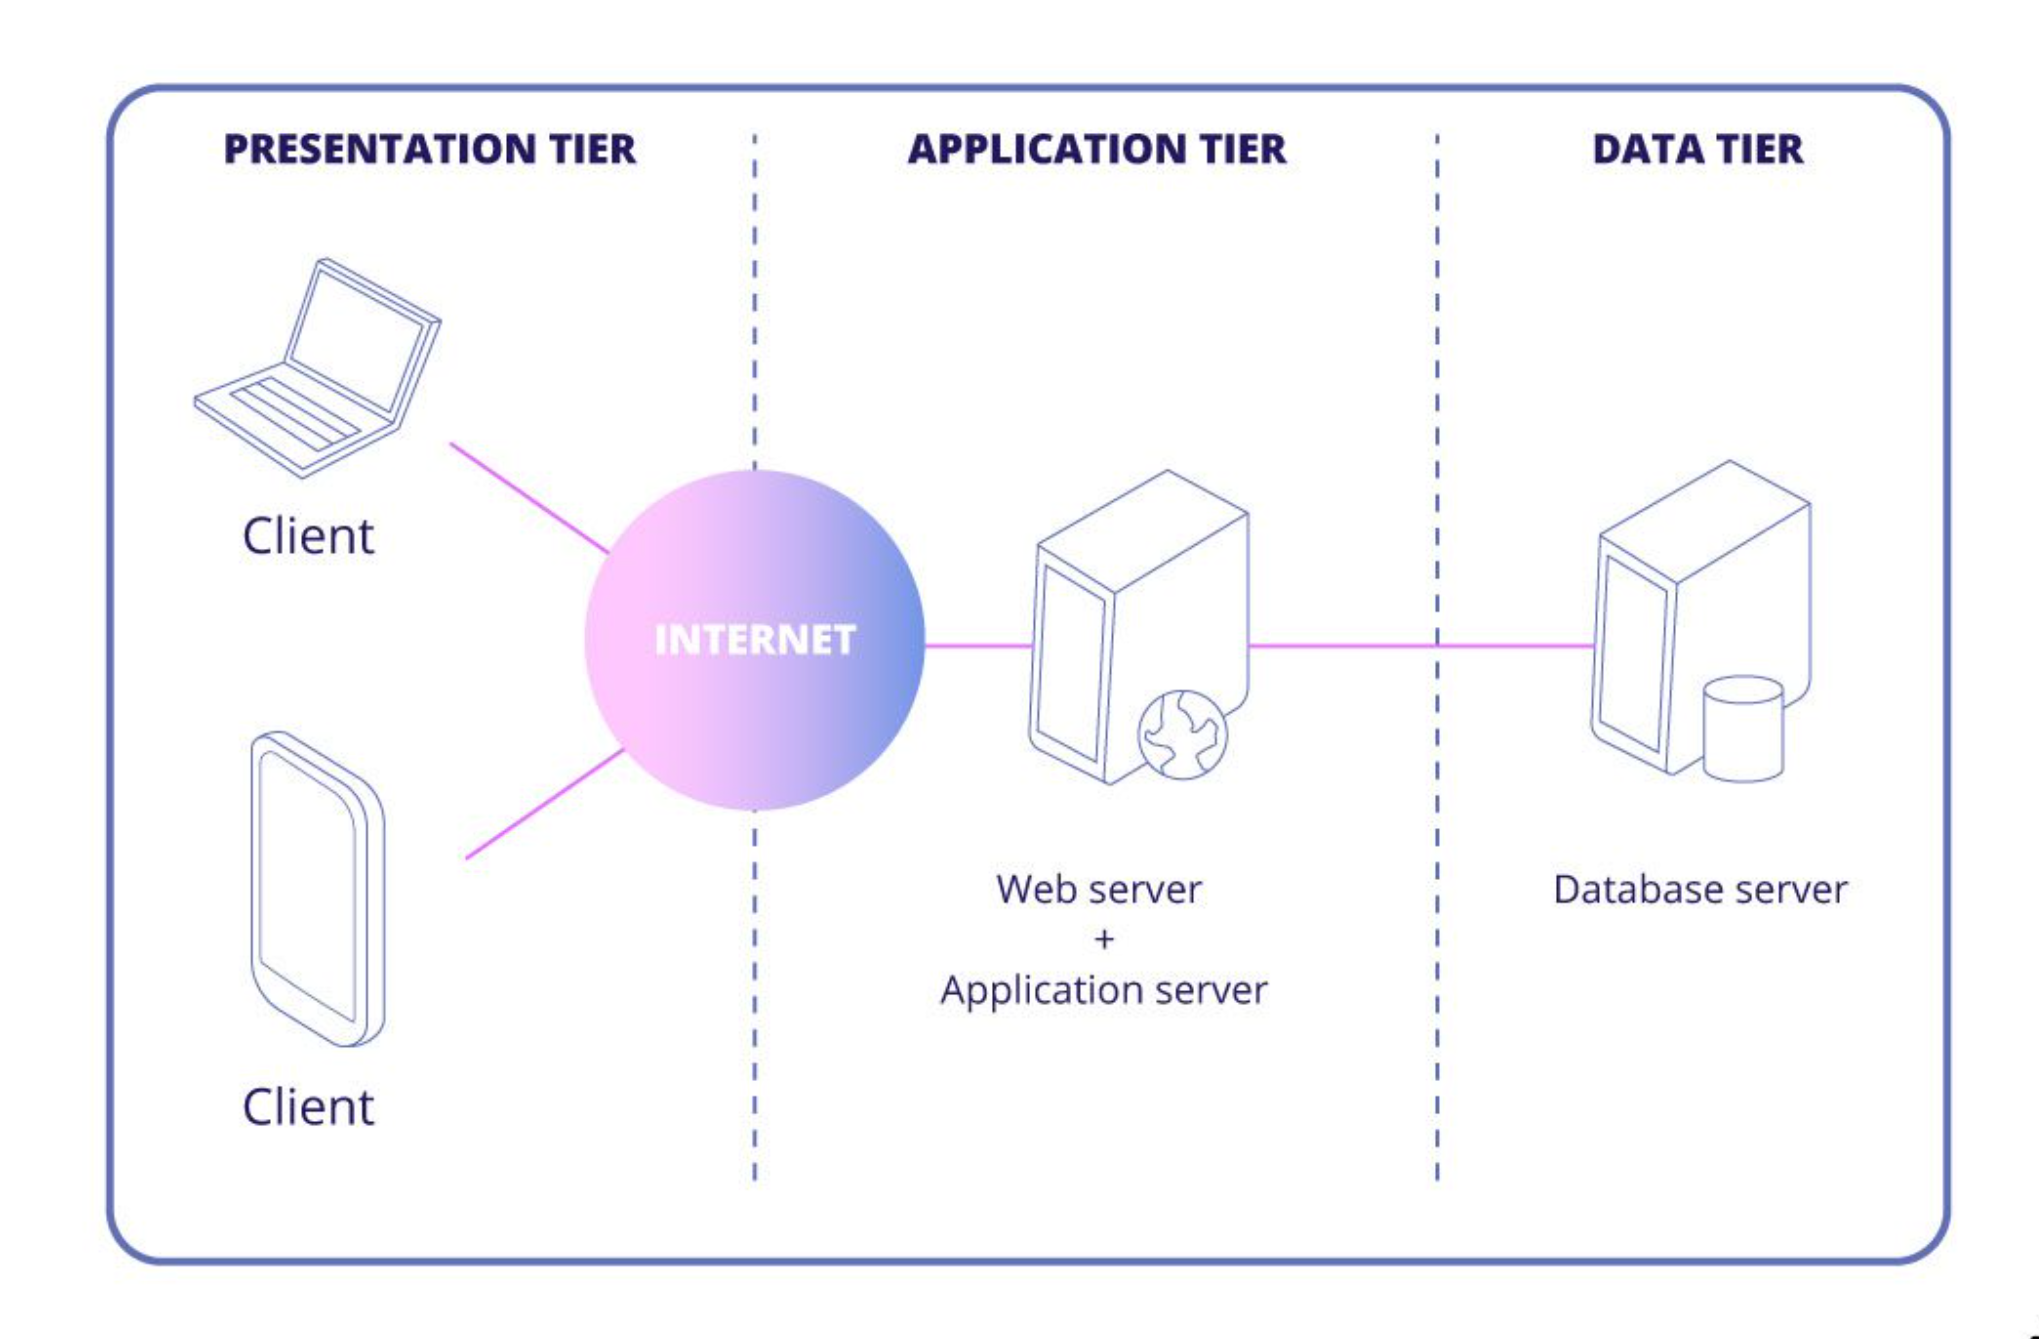
\includegraphics[width=100mm, scale=1]{figs/threetier.png}
    \caption{Arhitectura 3-tier. Sursa~\cite{ThreeTier}}
	\label{fig:threetier}
\end{figure}
%%%%%%%%%%%%%%%%%%%%%%%%%%%%%%%%%%%%%%%%%%%%%%%%%%%%%%%%%%%%%%%%%%%%%%%%%%%%%%%%%%%%%%%%%%%%%%%%%%%%%%%%%%%%%%%%%%%%%%%%%%%%%%%%%%%%%%%%%%%%
\subsection{Mediator Design Pattern}
Scopul utilizării acestui design pattern este de a reduce dependințele dintre obiecte, restricționând comunicarea între obiecte și mijlocind colaborarea printr-un mediator. \\

\noindent Avantajele utilizării mediatorului sunt:
\begin{itemize}
	\setlength\itemsep{0.5em}
    \item Comunicarea între mai multe componente poate fi extrasă într-un singur loc, fiind mai ușor de înțeles și modificat, acolo unde e cazul (Single Responsability Principle)
    \item Se pot introduce noi mediatori fără a schimba componentele deja existente
    \item Cuplarea între componente este redusă {\it (Low coupling)}
\end{itemize}
\begin{figure}[H]
	\centering
	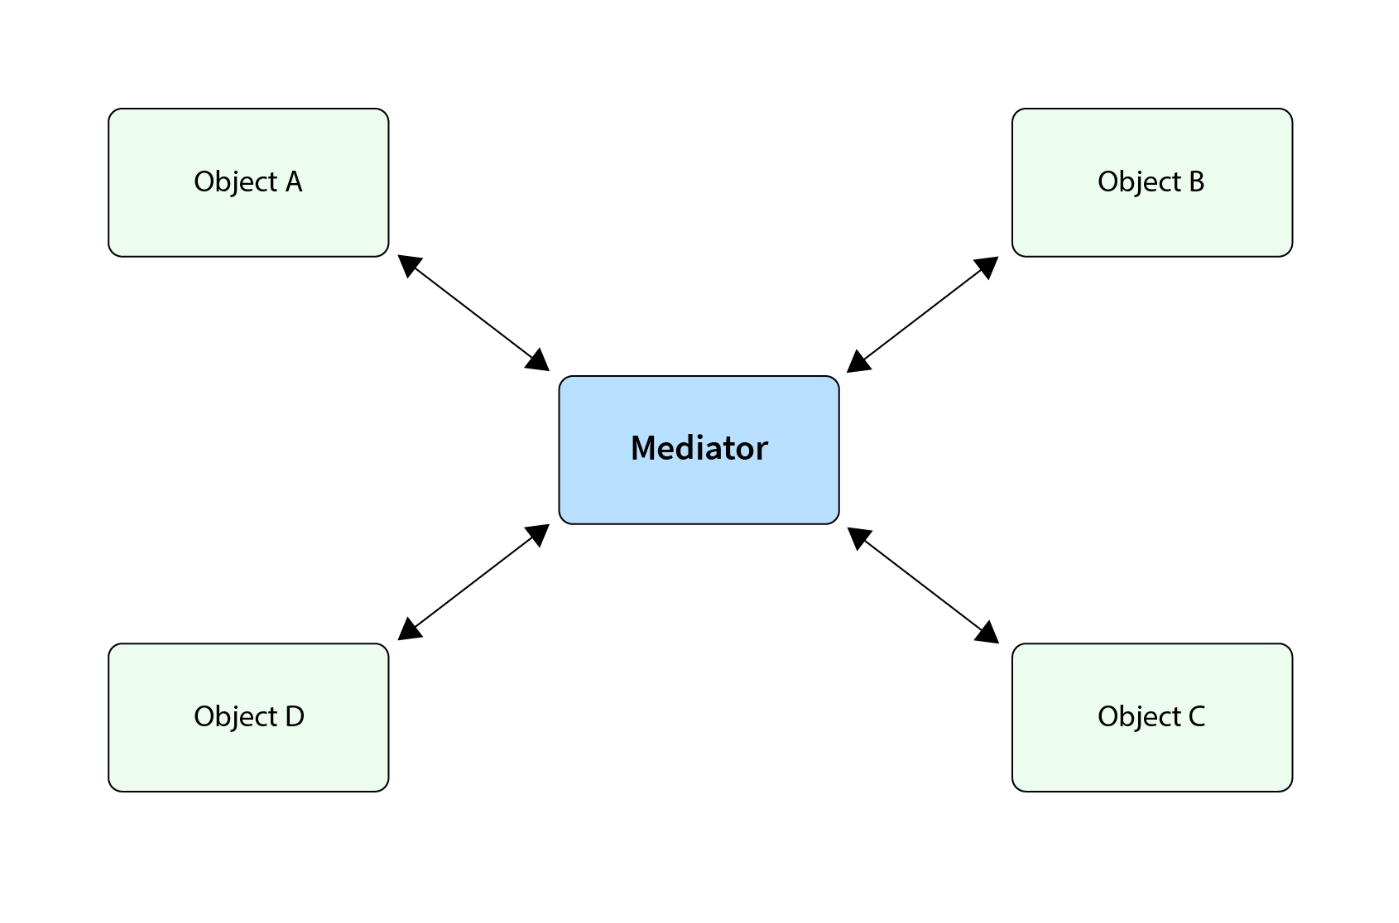
\includegraphics[width=100mm, scale=1]{figs/mediator.png}
    \caption{Diagramă Mediator Design Pattern. Sursa~\cite{Mediator}}
	\label{fig:mediator}
\end{figure}
%%%%%%%%%%%%%%%%%%%%%%%%%%%%%%%%%%%%%%%%%%%%%%%%%%%%%%%%%%%%%%%%%%%%%%%%%%%%%%%%%%%%%%%%%%%%%%%%%%%%%%%%%%%%%%%%%%%%%%%%%%%%%%%%%%%%%%%%%%%%
\subsection{CQRS}
Command-Query Responsibility Segregation sau CQRS este un design pattern care separă comenzile de interogări.\\
Comenzile sunt cele care scriu sau actualizează date în baza de date, iar o interogare citește datele din baza de date.
 
\begin{figure}[H]
	\centering
	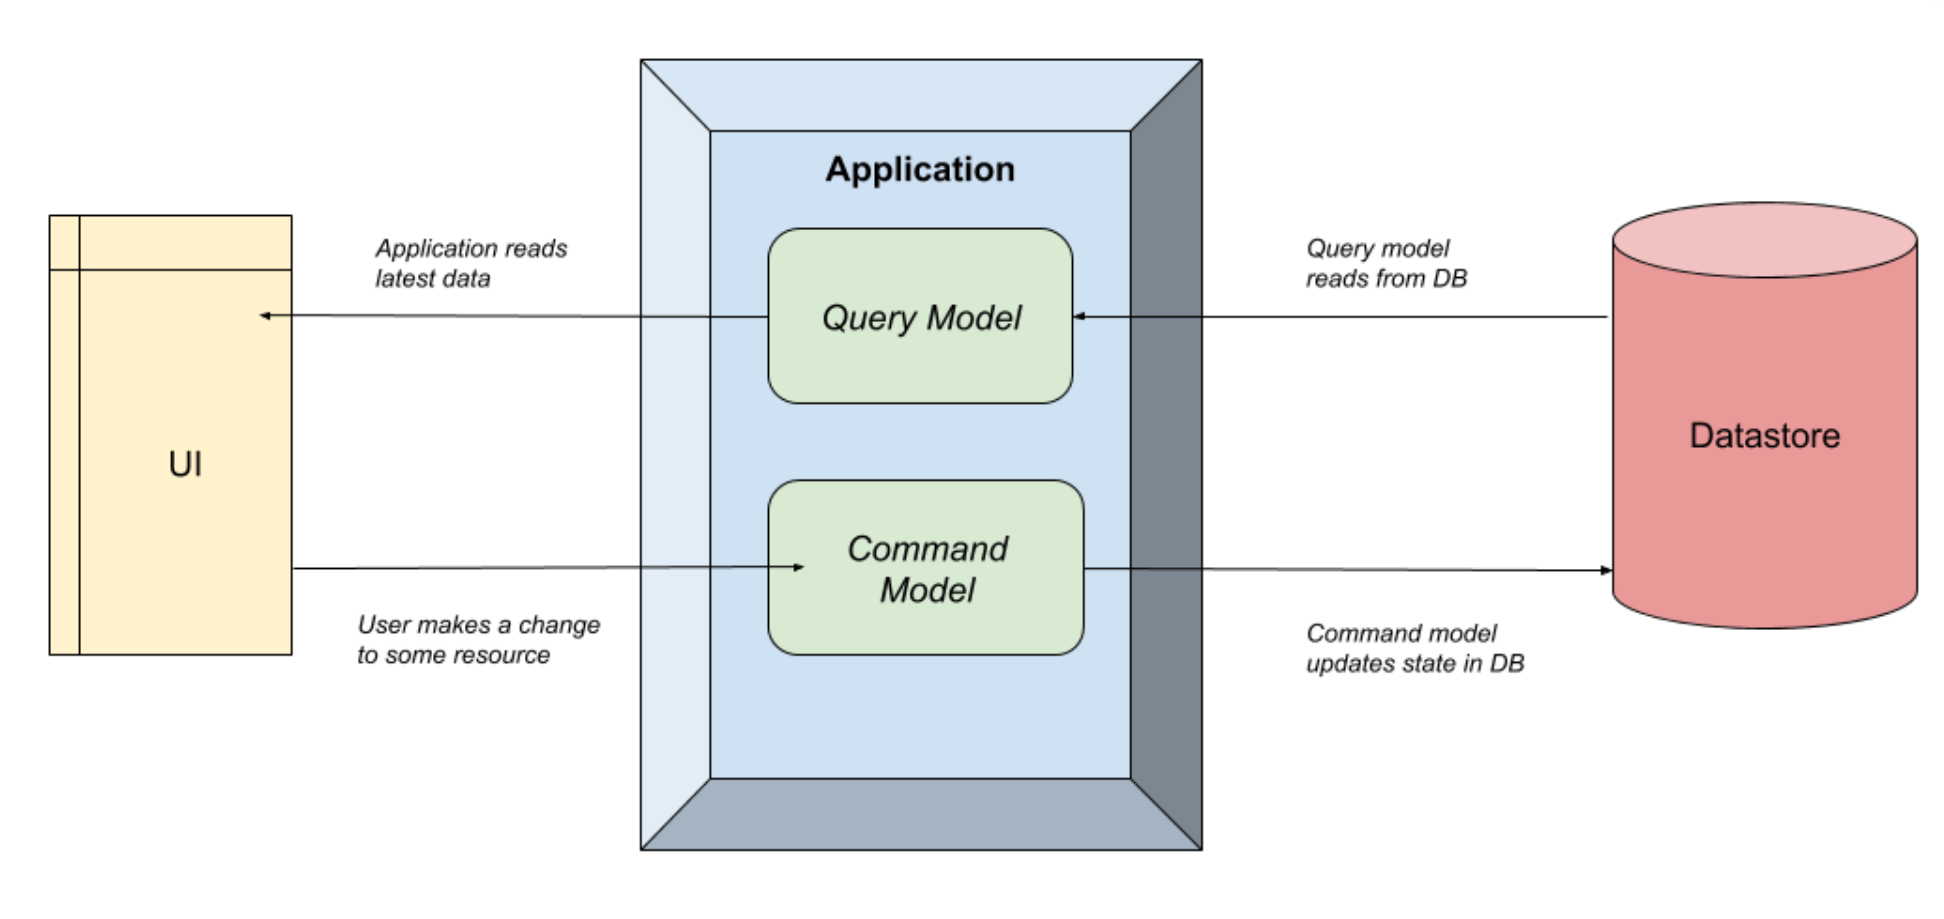
\includegraphics[width=100mm, scale=2]{figs/cqrs.png}
    \caption{Diagramă CQRS. Sursa~\cite{CQRS}}
	\label{fig:cqrs}
\end{figure}
%%%%%%%%%%%%%%%%%%%%%%%%%%%%%%%%%%%%%%%%%%%%%%%%%%%%%%%%%%%%%%%%%%%%%%%%%%%%%%%%%%%%%%%%%%%%%%%%%%%%%%%%%%%%%%%%%%%%%%%%%%%%%%%%%%%%%%%%%%%%
\subsection{Fluent Validation}
Fluent Validation este o librarie  din .NET pentru validarea modelelor. \\ 
Avantajul folosirii acestei librarii constă în faptul că logica de validare poate fi separată de modele și se renunță la adnotări.

În exemplul din figura \ref{fig:fluentValidation}, câmpul de firstName a fost completat cu un string gol, deși în validator modelul trebuie să aibă acest câmp este marcat ca fiind {\it required}.
De asemenea, a fost adăugată o validare extra pentru numărul de caractere și, fiind încălcată, este menționată în răspunsul din Swagger.
\begin{figure}[H]
	\centering
	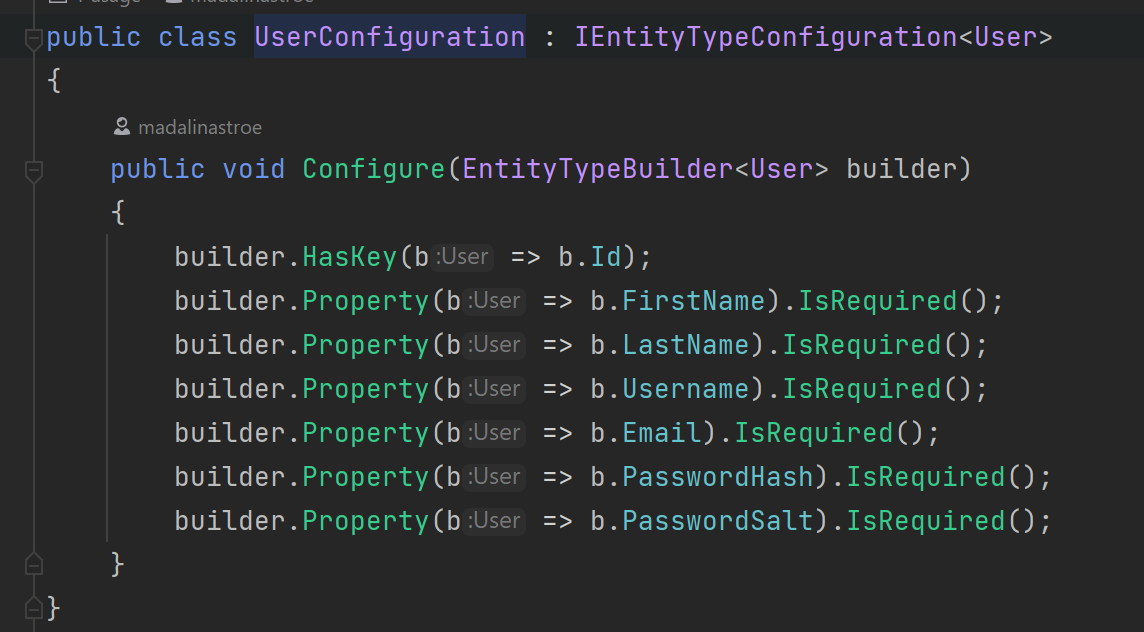
\includegraphics[width=100mm, scale=2]{figs/userConfigValidation.png}
	\caption{Configurare validări pentru modelul unui utilizator}
	\label{fig:userConfigValidation}
\end{figure}

\begin{figure}[H]
	\centering
	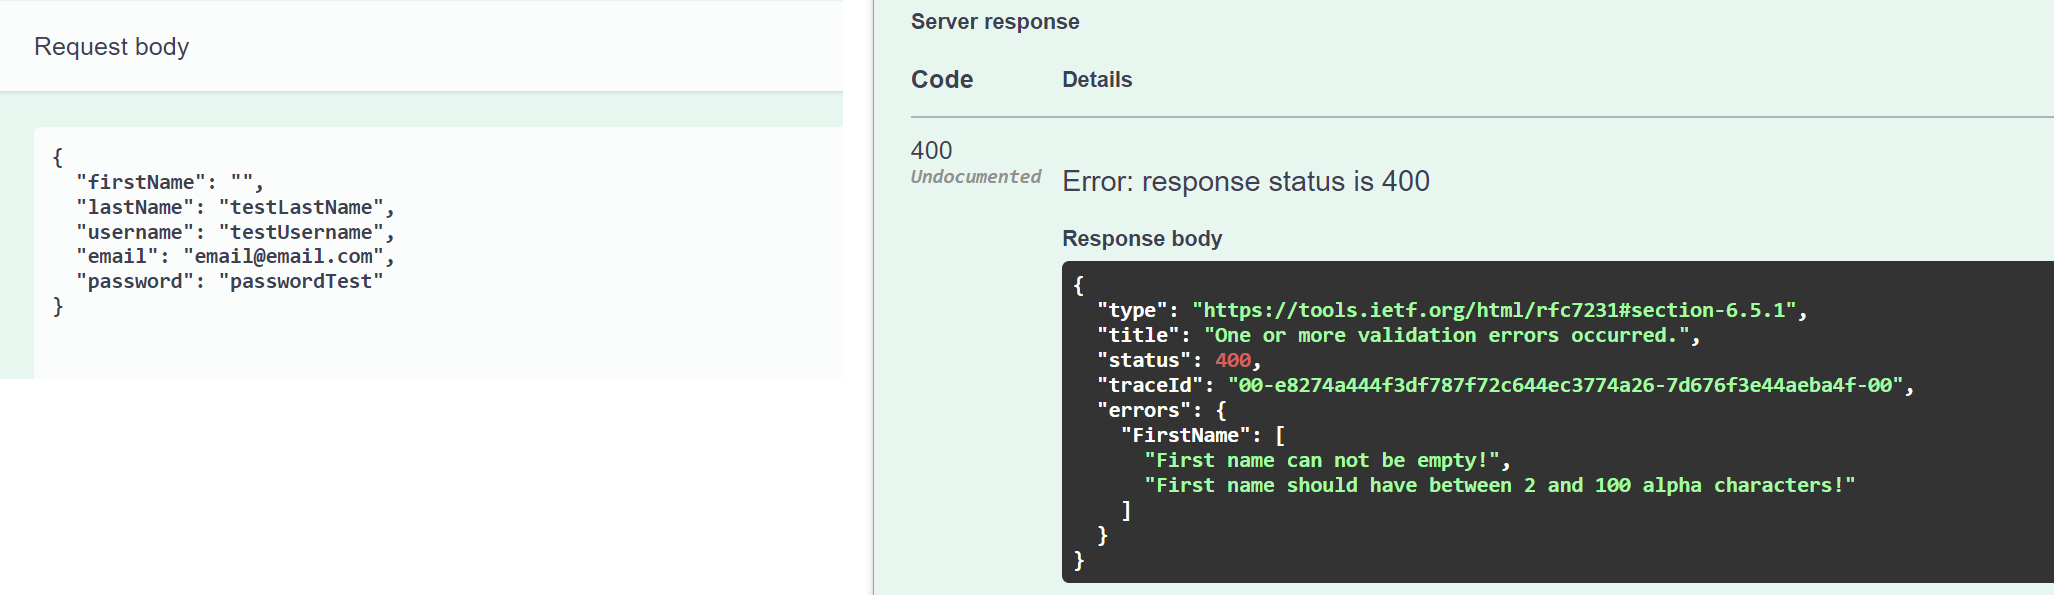
\includegraphics[width=150mm]{figs/fluentValidations.png}
	\caption{Request - Response folosind Fluent Validation}
	\label{fig:fluentValidation}
\end{figure}
%%%%%%%%%%%%%%%%%%%%%%%%%%%%%%%%%%%%%%%%%%%%%%%%%%%%%%%%%%%%%%%%%%%%%%%%%%%%%%%%%%%%%%%%%%%%%%%%%%%%%%%%%%%%%%%%%%%%%%%%%%%%%%%%%%%%%%%%%%%%
\section{Modul frontend}
\subsection{React}
Este un framework pentru dezvoltarea interfeței utilizator. Cu ajutorul acesteia, codul scris și componentele devin reutilizabile.\\
A fost dezvoltat de Facebook în 2011 și este cel mai popular framework din acest moment. 
Avantajele folosirii React sunt: 
\begin{itemize}
	\setlength\itemsep{0.5em}
    \item Ușor de învățat și folosit
    \item Componentele sunt reutilizabile
    \item Oferă flexibilitate
    \item SEO friendly
\end{itemize}

\begin{figure}[H]
	\centering
	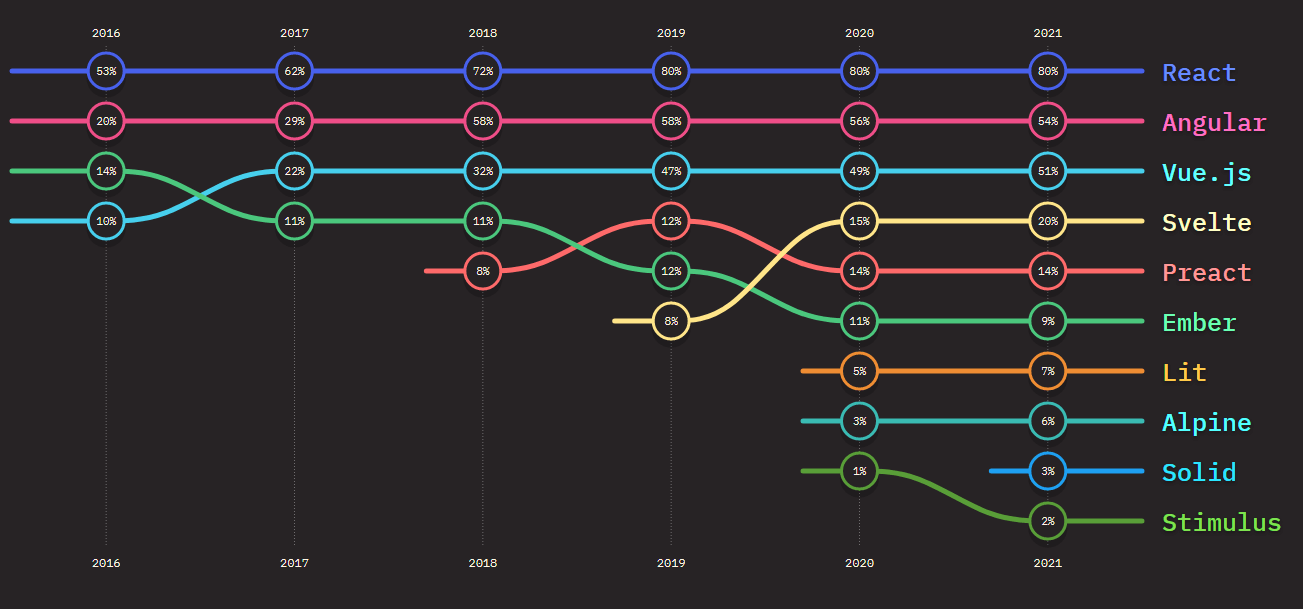
\includegraphics[width=100mm, scale=2]{figs/uiFrameworks.png}
    \caption{Cele mai populare frameworkuri pentru UI. Sursa~\cite{UIPopularity}}
    \label{fig:uiFrameworks}
\end{figure}
%%%%%%%%%%%%%%%%%%%%%%%%%%%%%%%%%%%%%%%%%%%%%%%%%%%%%%%%%%%%%%%%%%%%%%%%%%%%%%%%%%%%%%%%%%%%%%%%%%%%%%%%%%%%%%%%%%%%%%%%%%%%%%%%%%%%%%%%%%%%
\subsection{Ant Design}
Este o librărie din React, care conține componente ușor de utilizat.
Componentele pot fi customizate cu ajutorul designului oferit de librarie, dar și din exterior, cu ajutorul CSS.
Avantajele folosirii acestei librării sunt: 
\begin{itemize}
	\setlength\itemsep{0.5em}
    \item Design-ul consistent și accesibil
    \item Suport pentru Typescript și Javascript
    \item Form-uri ușor de customizat
    \item Variații pentru fiecare component
\end{itemize}
%%%%%%%%%%%%%%%%%%%%%%%%%%%%%%%%%%%%%%%%%%%%%%%%%%%%%%%%%%%%%%%%%%%%%%%%%%%%%%%%%%%%%%%%%%%%%%%%%%%%%%%%%%%%%%%%%%%%%%%%%%%%%%%%%%%%%%%%%%%%
\subsection{Styled Components}
Folosind CSS-in-JS, cu ajutorul librarie styled-components, componentele pot fi ajustate aplicând direct un stil customizat.
Avantajele folosirii sunt:
\begin{itemize}
	\setlength\itemsep{0.5em}
    \item Reutilizarea - precum componentele din React, pentru a evita duplicarea, acesta poate fi reutilizabil atunci când se aplică pe componente
    \item CSS
    \item Generează nume unice pentru fiecare clasa pentru targetarea corectă a componentelor
\end{itemize}

\begin{figure}[ht]
	\centering
	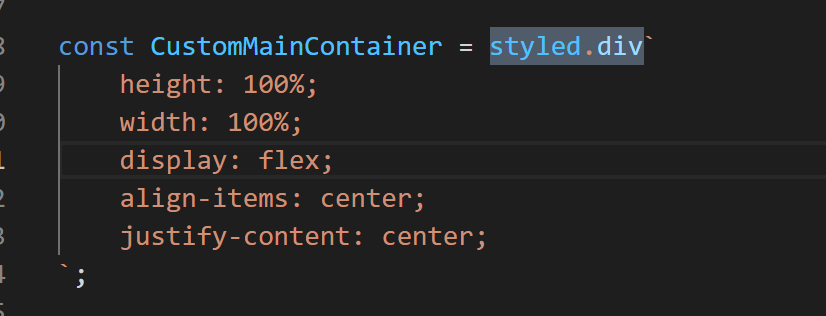
\includegraphics[width=100mm, scale=2]{figs/styledcomp.png}
	\caption{Exemplu utilizare styled-components}
	\label{fig:styledcomp}
\end{figure}
%%%%%%%%%%%%%%%%%%%%%%%%%%%%%%%%%%%%%%%%%%%%%%%%%%%%%%%%%%%%%%%%%%%%%%%%%%%%%%%%%%%%%%%%%%%%%%%%%%%%%%%%%%%%%%%%%%%%%%%%%%%%%%%%%%%%%%%%%%%%
\subsection{i18n}
Librăria i18next este folosită pentru internaționalizarea proiectului; mai exact, cu ajutorul acesteia rezolvăm partea de traducere a aplicației.\\
În acest fel, foarte simplu, tot conținutul aplicației poate fi schimbat în limba dorită, dacă sunt adăugate traducerile corespunzătoare.
%%%%%%%%%%%%%%%%%%%%%%%%%%%%%%%%%%%%%%%%%%%%%%%%%%%%%%%%%%%%%%%%%%%%%%%%%%%%%%%%%%%%%%%%%%%%%%%%%%%%%%%%%%%%%%%%%%%%%%%%%%%%%%%%%%%%%%%%%%%%
\section{Modele de Procesare a limbajului natural}
\subsection{FinBERT}
Bidirectional Encoder Representations from Transformers sau BERT este unul dintre cele mai folosite modele în Procesarea de Limbaj Natural din ultimii ani.
Este diferit față de modelele din anii anteriori, având un mecanism de self-attention, procesând textul bidirecțional.\\

Ce reprezintă un mecanism {\it self-attention}? În secțiunea "Self-Attention at a High Level" din~\cite{IllustratedTransformer},
rezumând câteva idei principale din publicația Attention Is All You Need~\cite{TransformerModel}, self-attention este o metodă folosită pentru a "privi" alte cuvinte relevante din enunț în timpul procesării cuvântului curent.
Bert~\cite{BERT} se bazează pe arhitectura Transformer~\cite{TransformerModel}, un model care a apărut în 2017, care depinde de aproximativ o sută de milioane de parametri.\\

\noindent Arhitectura Transformer, în figura \ref{fig:transformersArch}, este compusă din următoarele părți: 
\begin{itemize}
    \setlength\itemsep{0.5em}
    \item Tokenizarea textului
    \item Codificarea poziționala care injectează informații despre poziția inputului
    \item Codificarea contextuală a secvenței de intrare, pe nivelul de self-attention
    \item Nivelul feed forward care funcționează ca o memorie statică, cheie-valoare
    \item Nivelul de cross-atention decodifică secvența de ieșire
\end{itemize}
\begin{figure}[ht]
	\centering
	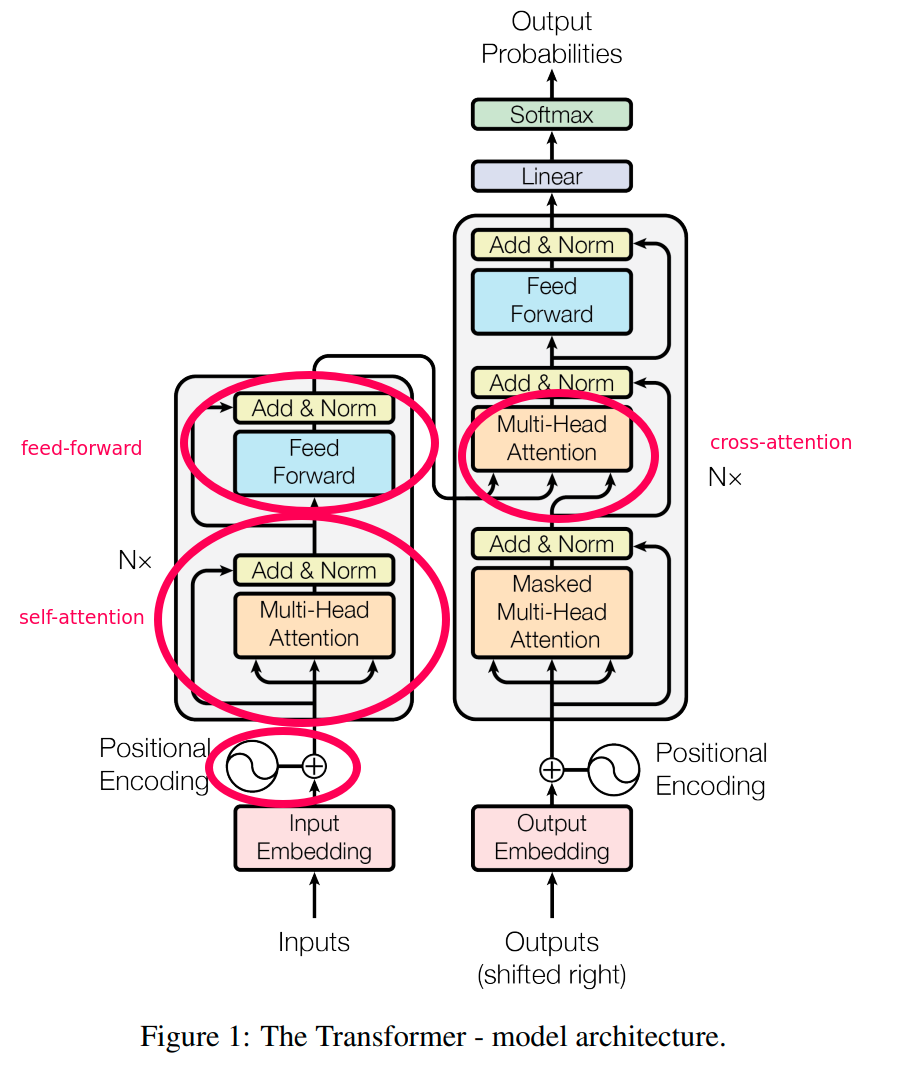
\includegraphics[width=100mm, scale=0.5]{figs/transformersArch.png}
    \caption{Arhitectura Transformers. Sursa~\cite{Transformers}}
	\label{fig:transformersArch}
\end{figure}
\ \\
În BERT, inputul este adus în primul nivel, apoi este transformat în alte codificări în următoarele nivele. 
Spre deosebire de abordările dinainte, prima etapă este etapa de pre-antrenare (en: pre-training), unde folosește 2 task-uri nesupervizate.
După această etapă, modelul poate să fie perfecționat pentru o sarcină specifică, precum analiza de sentimente. \\

Analiza de sentimente pentru un text reprezintă extragerea sentimentelor sau opiniilor oamenilor dintr-un text scris.
Analiza sentimentelor financiare diferă de analiza de sentimente prin scopul ei, pentru că rezultatul acestei analize va determina modul în care piața va fi influențată de deciziile financiare.\\
În~\cite{FinBERT1}, autorii spun despre FinBERT că este un model de analiză a textului bazat pe BERT, cu un domeniu specific. Acest model a fost antrenat pe un corpus de 4.9 miliarde de tokeni compuși din rapoarte ale companiilor, transcripturi ale conferințelor și rapoarte de analiză, conform \cite{FinBERT2}.\\

În Statele Unite ale Americii, toate companiile cotate la bursă depun rapoarte anuale, cunoscute sub numele de Form 10-K și rapoarte trimestriale, cunoscute sub numele de 10-Q. Aceste documente sunt publice și oferă o imagine de ansamblu a situației financiare a companiei.\\
Cele menționate mai sus, alături de rapoarte ale analiștilor, care oferă măsuri rezumative cu recomandări, și teleconferințe trimestriale pe care directorii companiilor le au cu investitorii pentru a discuta despre performanța firmei, formează un corpus financiar. \\
Un corpus sau corpora reprezintă o colecție de texte sau fișiere audio organizate în seturi de date (en: datasets). Un corpus este, în general, folosit pentru antrenarea sistemelor bazate pe Inteligență Artificială. 
%%%%%%%%%%%%%%%%%%%%%%%%%%%%%%%%%%%%%%%%%%%%%%%%%%%%%%%%%%%%%%%%%%%%%%%%%%%%%%%%%%%%%%%%%%%%%%%%%%%%%%%%%%%%%%%%%%%%%%%%%%%%%%%%%%%%%%%%%%%%
\subsection{Sumarizator de text}
Sumarizarea este procesul de producere a unei versiuni mai scurte a unui text sau document, păstrând ideile importante din textul original.
Deși modelul BERT este folosit pentru multe task-uri de NLP, în diferite domenii și subdomenii, acesta nu este soluția și pentru sumarizarea textului sau traduceri. În acest caz, apare BART (Denoising Sequence-to-Sequence Pre-training for Natural
Language Generation, Translation, and Comprehension), care folosește arhitectura sequence-to-sequence din Transformers și este un model folosit pentru clasificarea și generarea textului.\\
Este implementat ca un model sequence-to-sequence cu un codificator bidirecțional pentru textul corupt și un decodificator stânga-dreapa.
Arhitectura este asemănătoare cu arhitectura BERT, cu câteva diferențe, menționate în ~\cite{BARTArchitecture}: 
\begin{itemize}
    \setlength\itemsep{0.5em}
    \item Fiecare nivel al decodificatorului efectuează suplimentar funcția de cross-atention pe ultimul strat ascuns al codificatorului
    \item BERT folosește o rețea feed-forward suplimentară, spre deosebire de BART
\end{itemize}
\ \\
Acest model este pre-antrenat folosind un framework {\it Corrupt and Reconstruct}~\cite{CorruptAndReconstruct} care ia un text, aplică o funcție de zgomot, apoi antrenează modelul să reconstruiască textul original. 
Printre funcțiile de zgomot avem: 
\begin{itemize}
    \setlength\itemsep{0.5em}
    \item Mascarea tokenilor (Token Masking) - se maschează anumiți token și se încearcă reconstrucția textului original
    \item Ștergerea tokenilor (Token deletion) - se șterg anumiți token și se încearcă reconstrucția textului original
    \item Rotația documentului (Document Rotation) - Mutarea anumitor tokeni pentru ca modelul să identifice începutul secvenței
    \item Permutarea enunțului (Sentence Permutation) - Se iau toate frazele din document și sunt amestecate
    \item Completarea texului (Text infilling) - Un număr fix de tokeni este șters și înlocuit cu o singură mască. Modelul învață să prezică numărul de tokeni ce lipsesc dintr-un span și conținutul acestora~\cite{SpanBERT}
\end{itemize}
\begin{figure}[H]
	\centering
	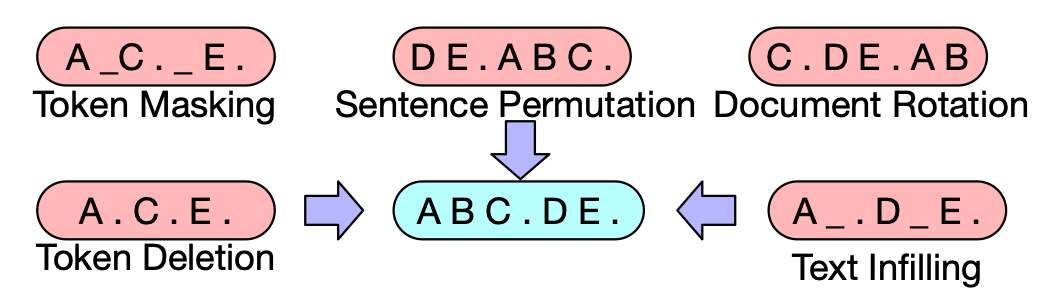
\includegraphics[width=100mm, scale=0.5]{figs/bartNoise.png}
    \caption{BART - Funcții de zgomot (Noising Functions). Sursa~\cite{BART}}
	\label{fig:bartNoise}
\end{figure}

BART este folosit pentru sumarizarea textului; în funcție de abordare, aceasta poate fi de două tipuri: abstractivă sau extractivă. \\
Sumarizarea extractivă identifică și extrage cele mai semnificative enunțuri din text, pe când, prin sumarizarea abstractivă,
se încearcă înțelegerea întregului text și generarea unui sumar cu un text parafrazat, cea de-a doua metodă fiind utilizată și de BART.
Modelul ales în acest proiect este bazat pe modelele DistilBART și este evaluat folosind metrica ROUGE~\cite{Rouge}, bazat pe suprapunerea dintre secvența produsă și secvența corectă. 
%%%%%%%%%%%%%%%%%%%%%%%%%%%%%%%%%%%%%%%%%%%%%%%%%%%%%%%%%%%%%%%%%%%%%%%%%%%%%%%%%%%%%%%%%%%%%%%%%%%%%%%%%%%%%%%%%%%%%%%%%%%%%%%%%%%%%%%%%%%%
\subsection{Keyphrase Extractor}
Extragerea de cuvinte sau fraze cheie reprezintă o tehnică prin care sunt extrase cuvintele părțile importante dintr-un text. \\
În~\cite{KBIR}, autorii spun că frazele sau cuvintele cheie captează cele mai importante idei și identificarea lor automată ajută foarte mult în sarcini precum clasificarea, sumarizarea, etc.
Modelul KBIR folosește o combinație de mascare a tokenilor (Masked Language Modeling - MLM), mascare a expresiilor (Keyphrase Bounday Infilling - KBI) și învățarea constrativă (Keyphrase Replacement Classification - KRC).

%%%%%%%%%%%%%%%%%%%%%%%%%%%%%%%%%%%%%%%%%%%%%%%%%%%%%%%%%%%%%%%%%%%%%%%%%%%%%%%%%%%%%%%%%%%%%%%%%%%%%%%%%%%%%%%%%%%%%%%%%%%%%%%%%%%%%%%%%%%%
\section{Aplicații similare}
În momentul de față, există destul de puține aplicații publice pentru analiza textelor financiare. 
\subsection{Serviciul de înțelegere a limbajului natural dezvoltat de IBM}
{\noindent Acest serviciu are următoarele funcționalități:}
\begin{itemize}
    \setlength\itemsep{0.5em}
    \item Analiza textului în mai multe domenii - Legal, Media și Financiar
    \item Textul analizat poate să fie copiat în field-ul din aplicație sau poate să fie referit prin URL
    \item Pentru partea de extracție din text, pot fi ca rezultat următoarele:
    \begin{itemize}
        \setlength\itemsep{0.5em}
        \item Entitațile extrase care pot aparține unui tip (ex: Organization, Job title, etc.)
        \item Cuvintele cheie extrase
        \item Conceptele extrase
        \item Relațiile dintre entitați
    \end{itemize}
    \item Pentru partea de clasificare a textului, pot fi ca rezultat următoarele:
    \begin{itemize}
        \setlength\itemsep{0.5em}
        \item Scorul sentimentului pe întregul document
        \item Scorul sentimentului pe fiecare entitate extrasă 
        \item Scorul sentimentului pe fiecare entitate cuvânt cheie sau frază 
        \item Clasificarea emoțiilor pe întregul document (ex: Sadness, Joy, Disgust, Fear, Anger, etc.)
        \item Clasificarea emoțiilor pentru fiecare entitate
        \item Clasificarea emoțiilor pentru fiecare cuvânt cheie sau frază
        \item Clasificarea în categorii, ierarhic
    \end{itemize}
    \item Pentru partea lingvistică a textului, pot fi ca rezultat următoarele:
    \begin{itemize}
        \setlength\itemsep{0.5em}
        \item Rolurile semantice (Subiect + Acțiune + Forma obiectului)
        \item Sintaxa - pentru fiecare token se specifică partea de vorbire
    \end{itemize}
\end{itemize}
\begin{figure}[H]
	\centering
	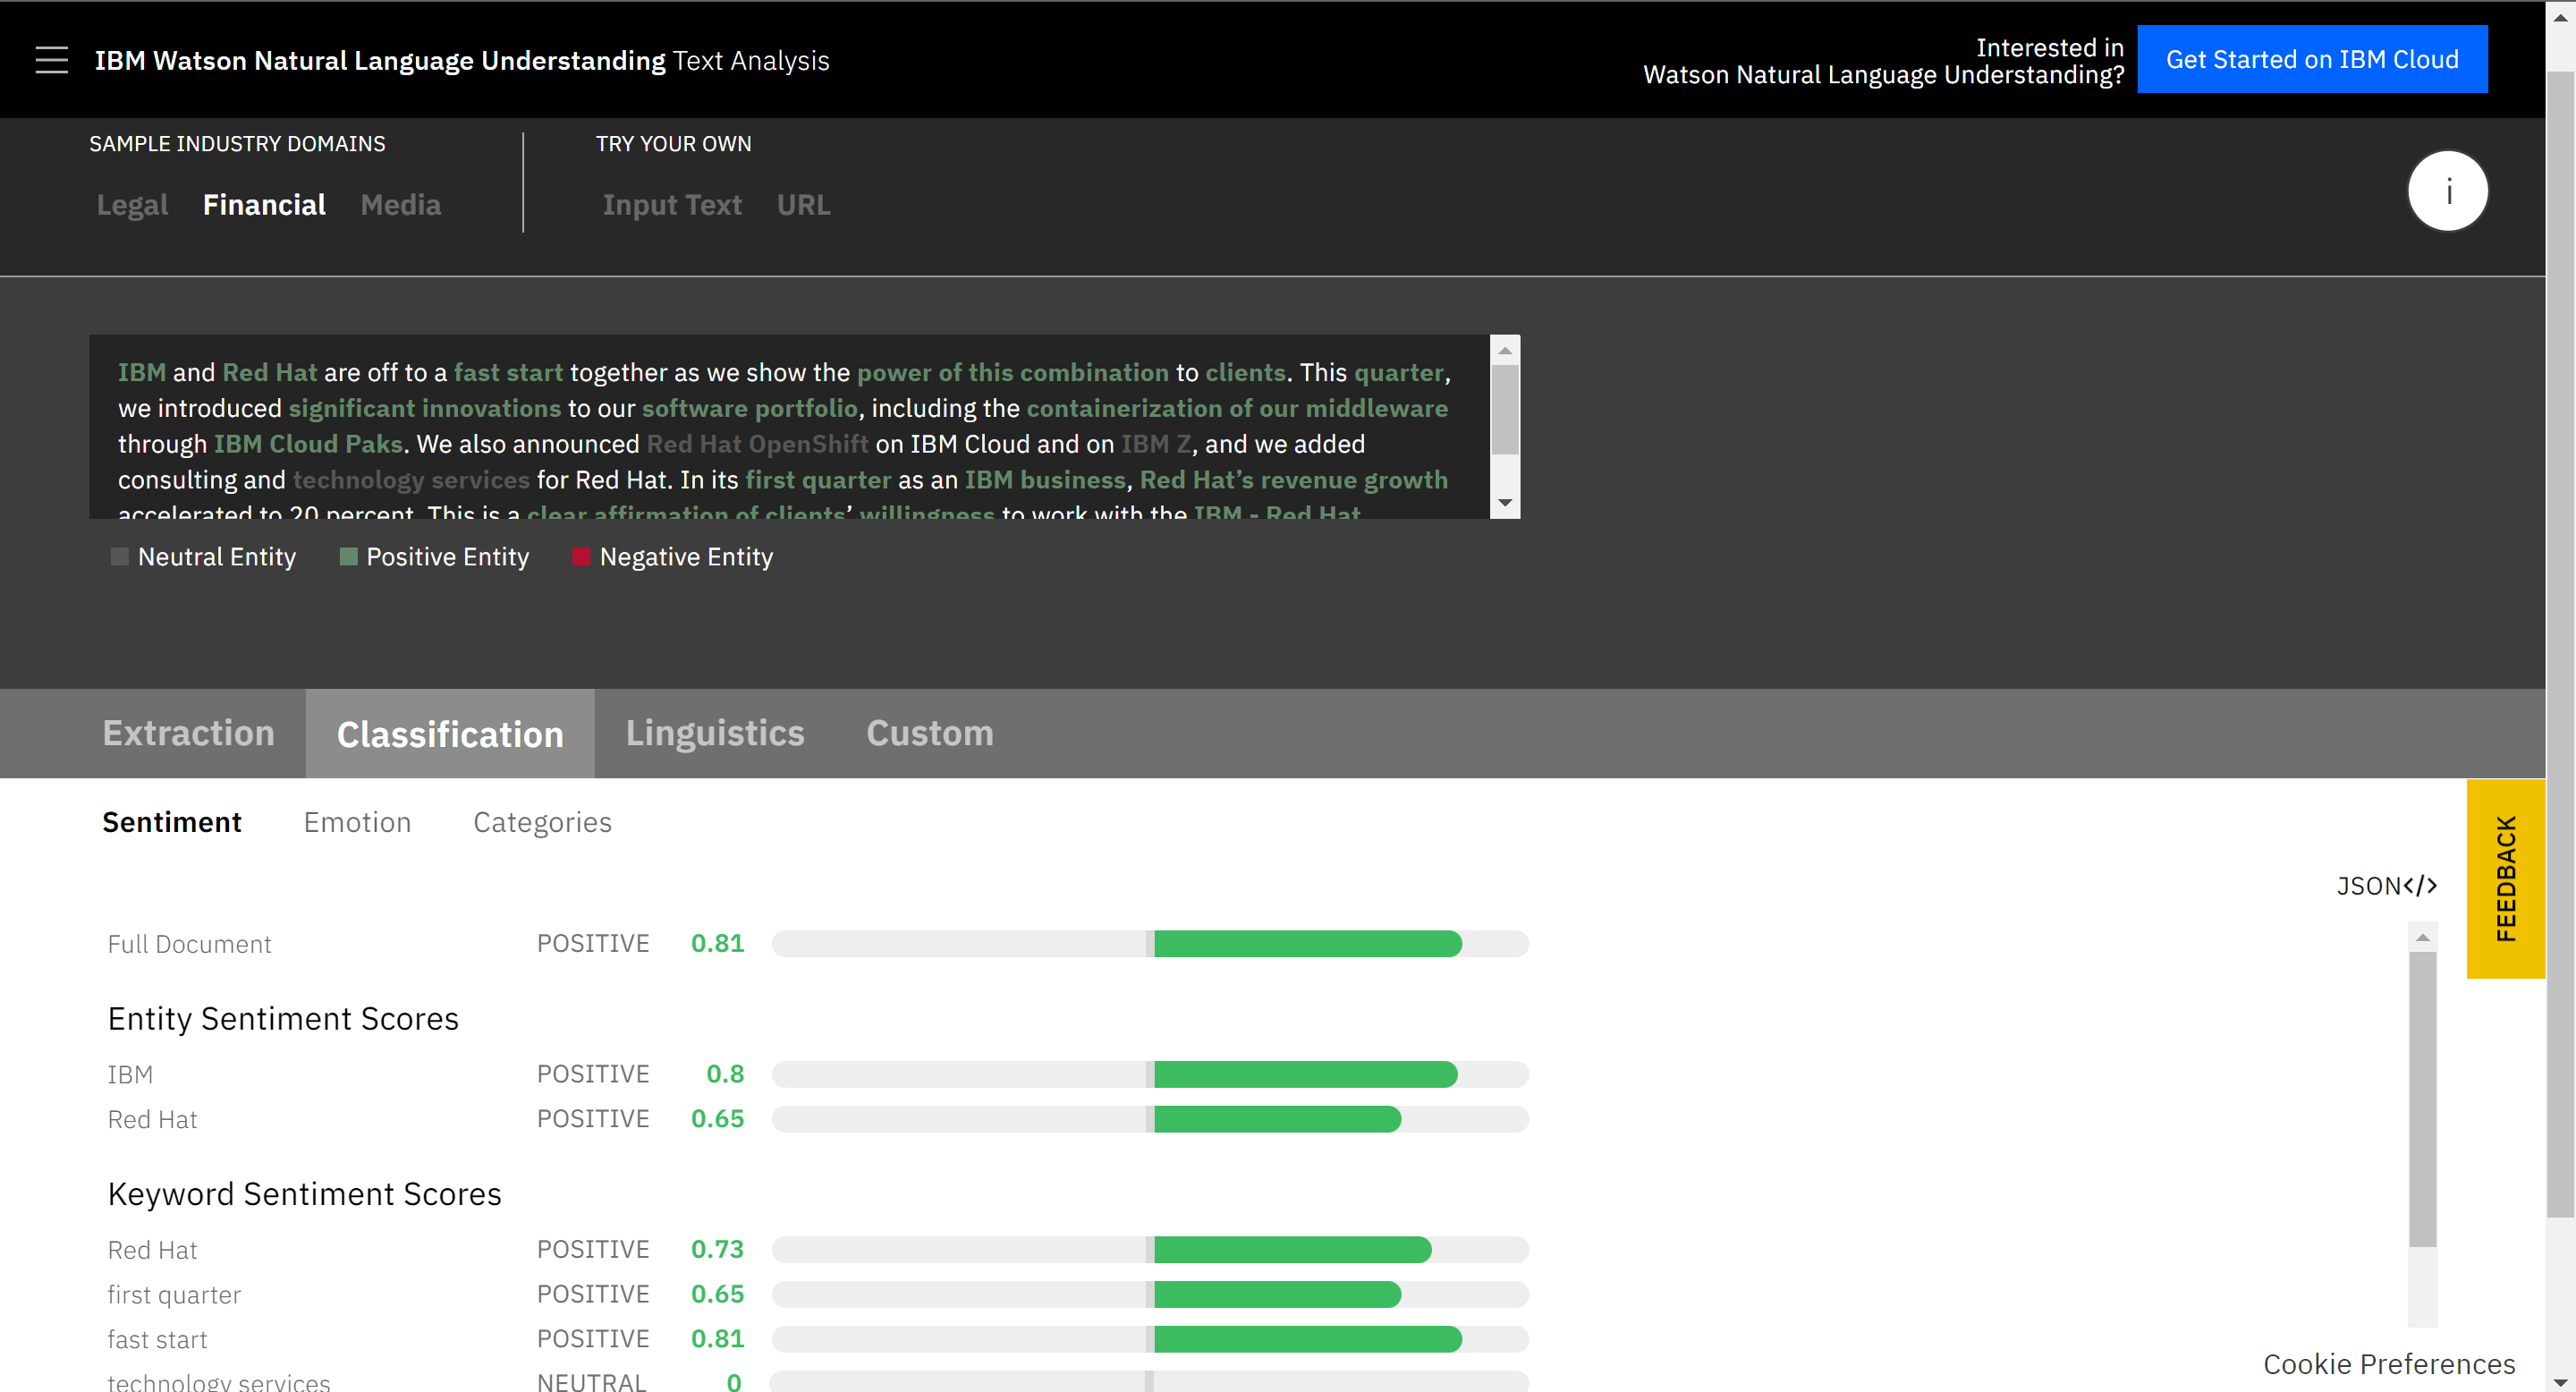
\includegraphics[width=150mm]{figs/ibmCloud.png}
    \caption{Servicii IBM}
	\label{fig:ibmCloud}
\end{figure}
\subsection{Google Cloud Natural Language}
{\noindent Acest serviciu are următoarele funcționalități:}
\begin{itemize}
    \setlength\itemsep{0.5em}
    \item Entitațile extrase care pot aparține unui tip (ex: Organization, Location, Person, Event, Other, etc.)
    \item Scorul sentimentului și magnitudinea pe întregul document
    \item Scorul sentimentului și magnitudinea pe fiecare entitate extrasă 
    \item Sintaxa - pentru fiecare token (inclusiv semne de punctuație) se specifică partea de vorbire(cu mai multe informații specifice pentru fiecare, spre exemplu, caz, gen, timp, număr),lemma, morfologia, etc.
    \item Clasificarea în categorii
\end{itemize}
\begin{figure}[H]
	\centering
	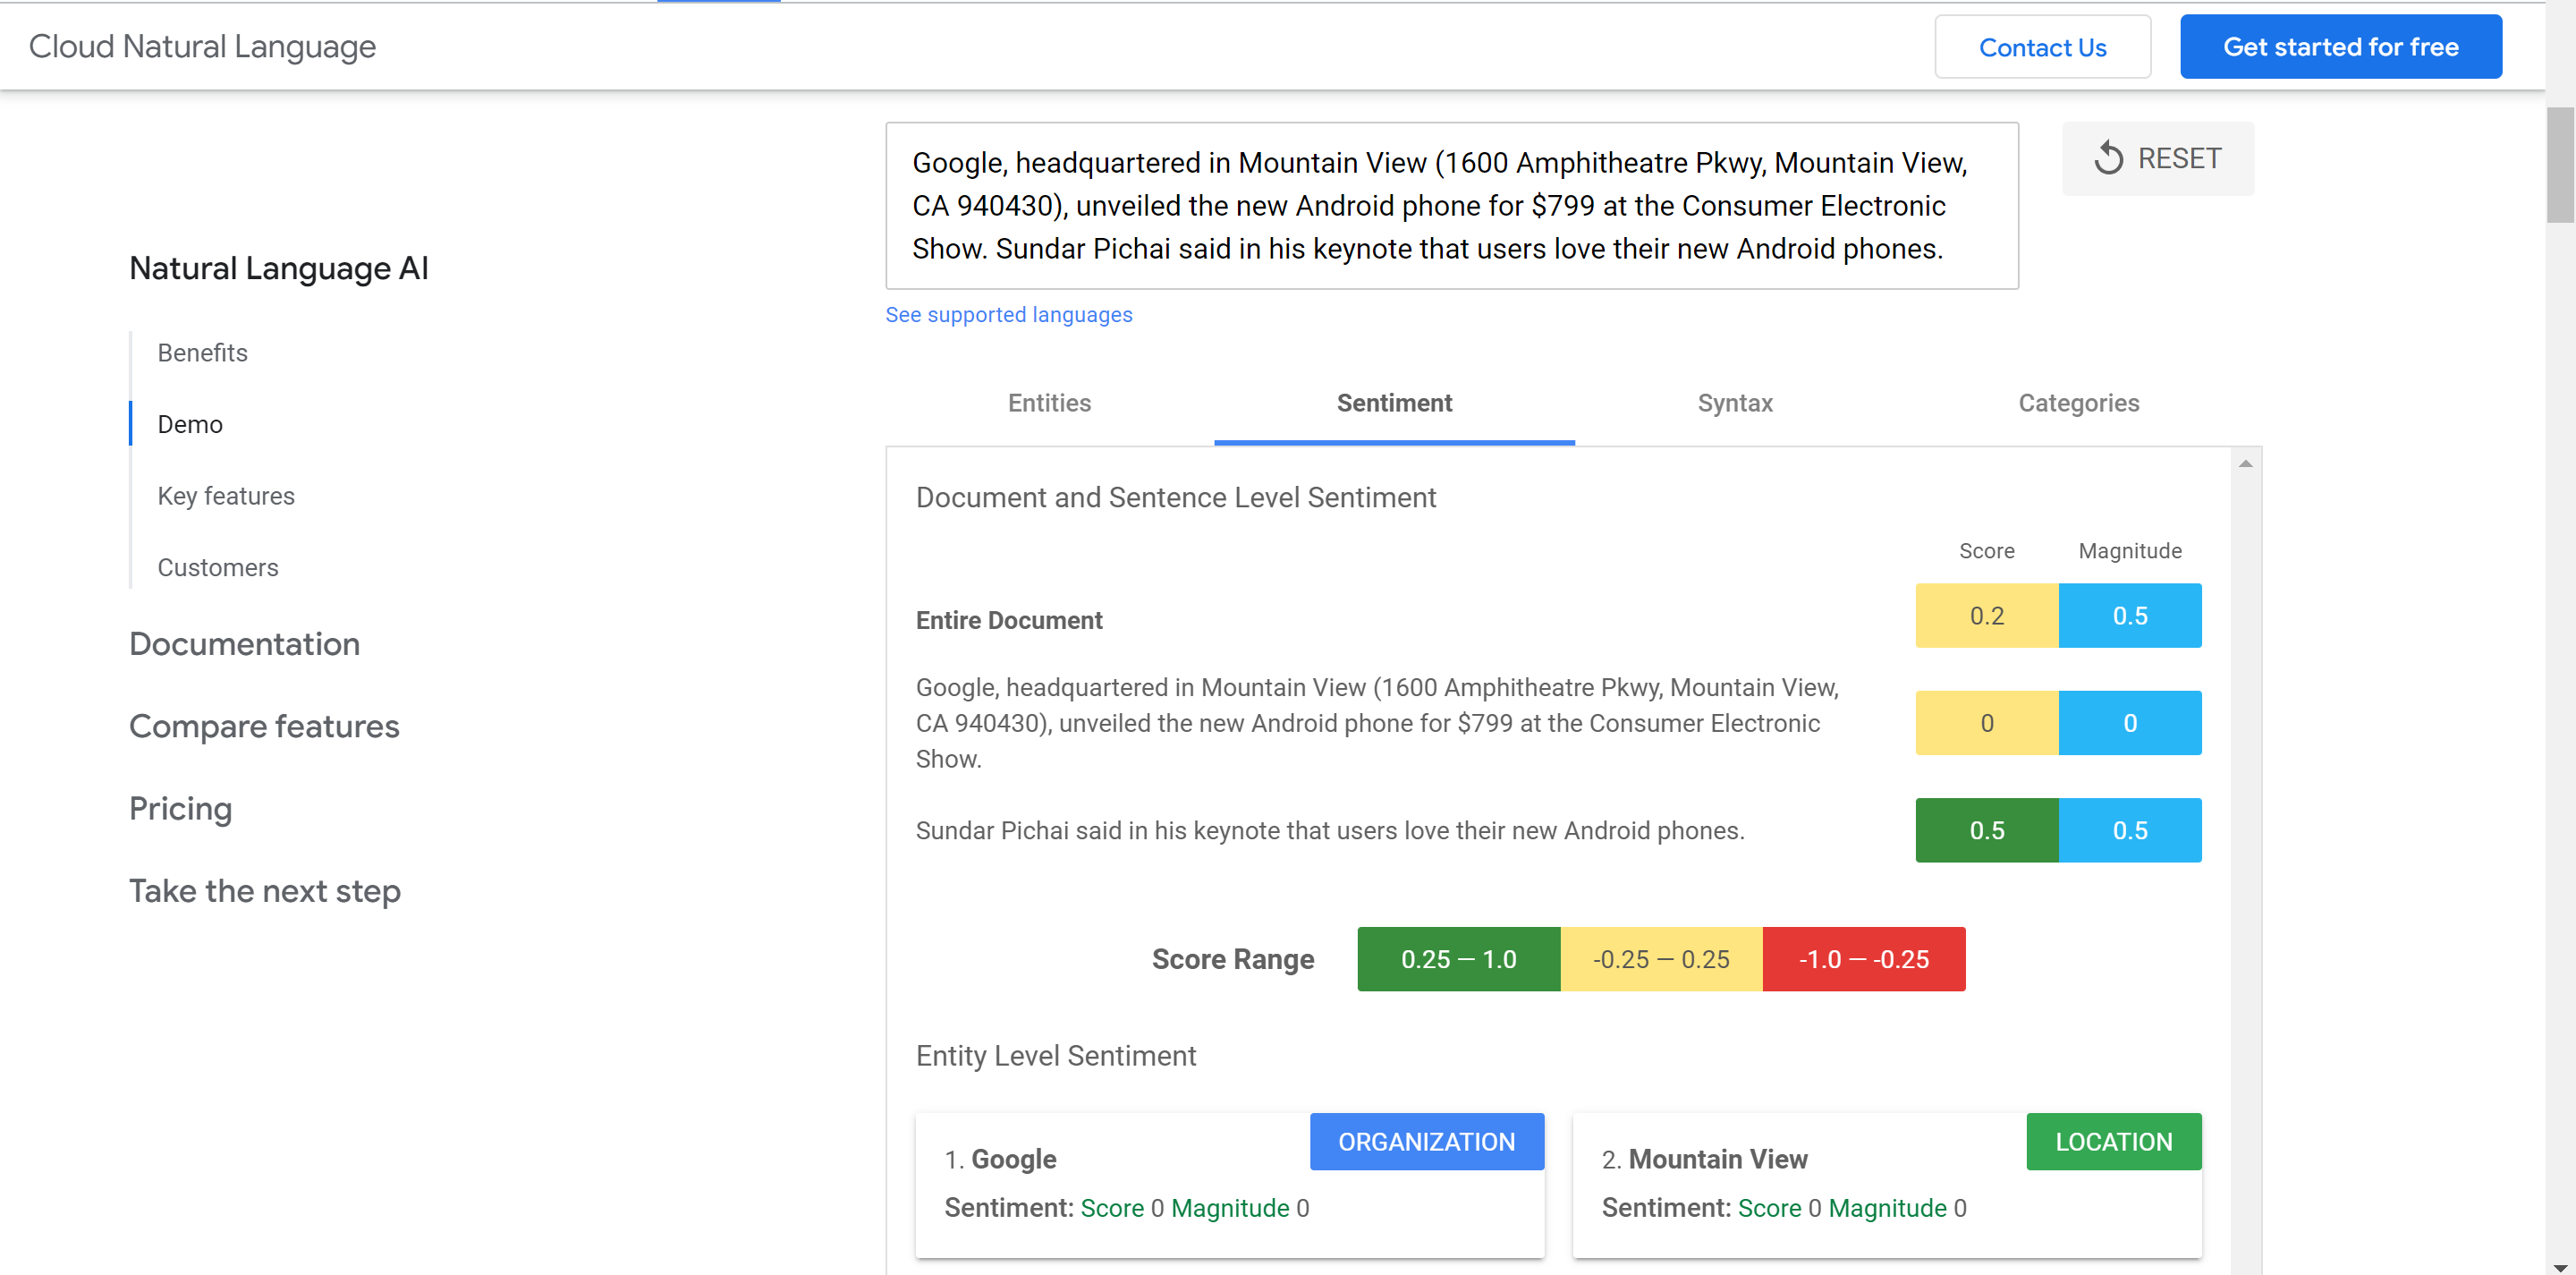
\includegraphics[width=150mm]{figs/googleSearch.png}
    \caption{Servicii Google Cloud Natural Language}
	\label{fig:googleSearch}
\end{figure}
\subsection{Microsoft AI}
{\noindent Acest serviciu are următoarele funcționalități:}
\begin{itemize}
    \setlength\itemsep{0.5em}
    \item Scorul sentimentului pe întreg textul
    \item Extracția entităților, iar acolo unde este posibil, fiecare entitate se află sub un link de Wikipedia
    \item Bing Entity Search oferă un sumar al informațiilor relevante pentru fiecare entitate găsită la punctul anterior
\end{itemize}
\begin{figure}[t]
	\centering
	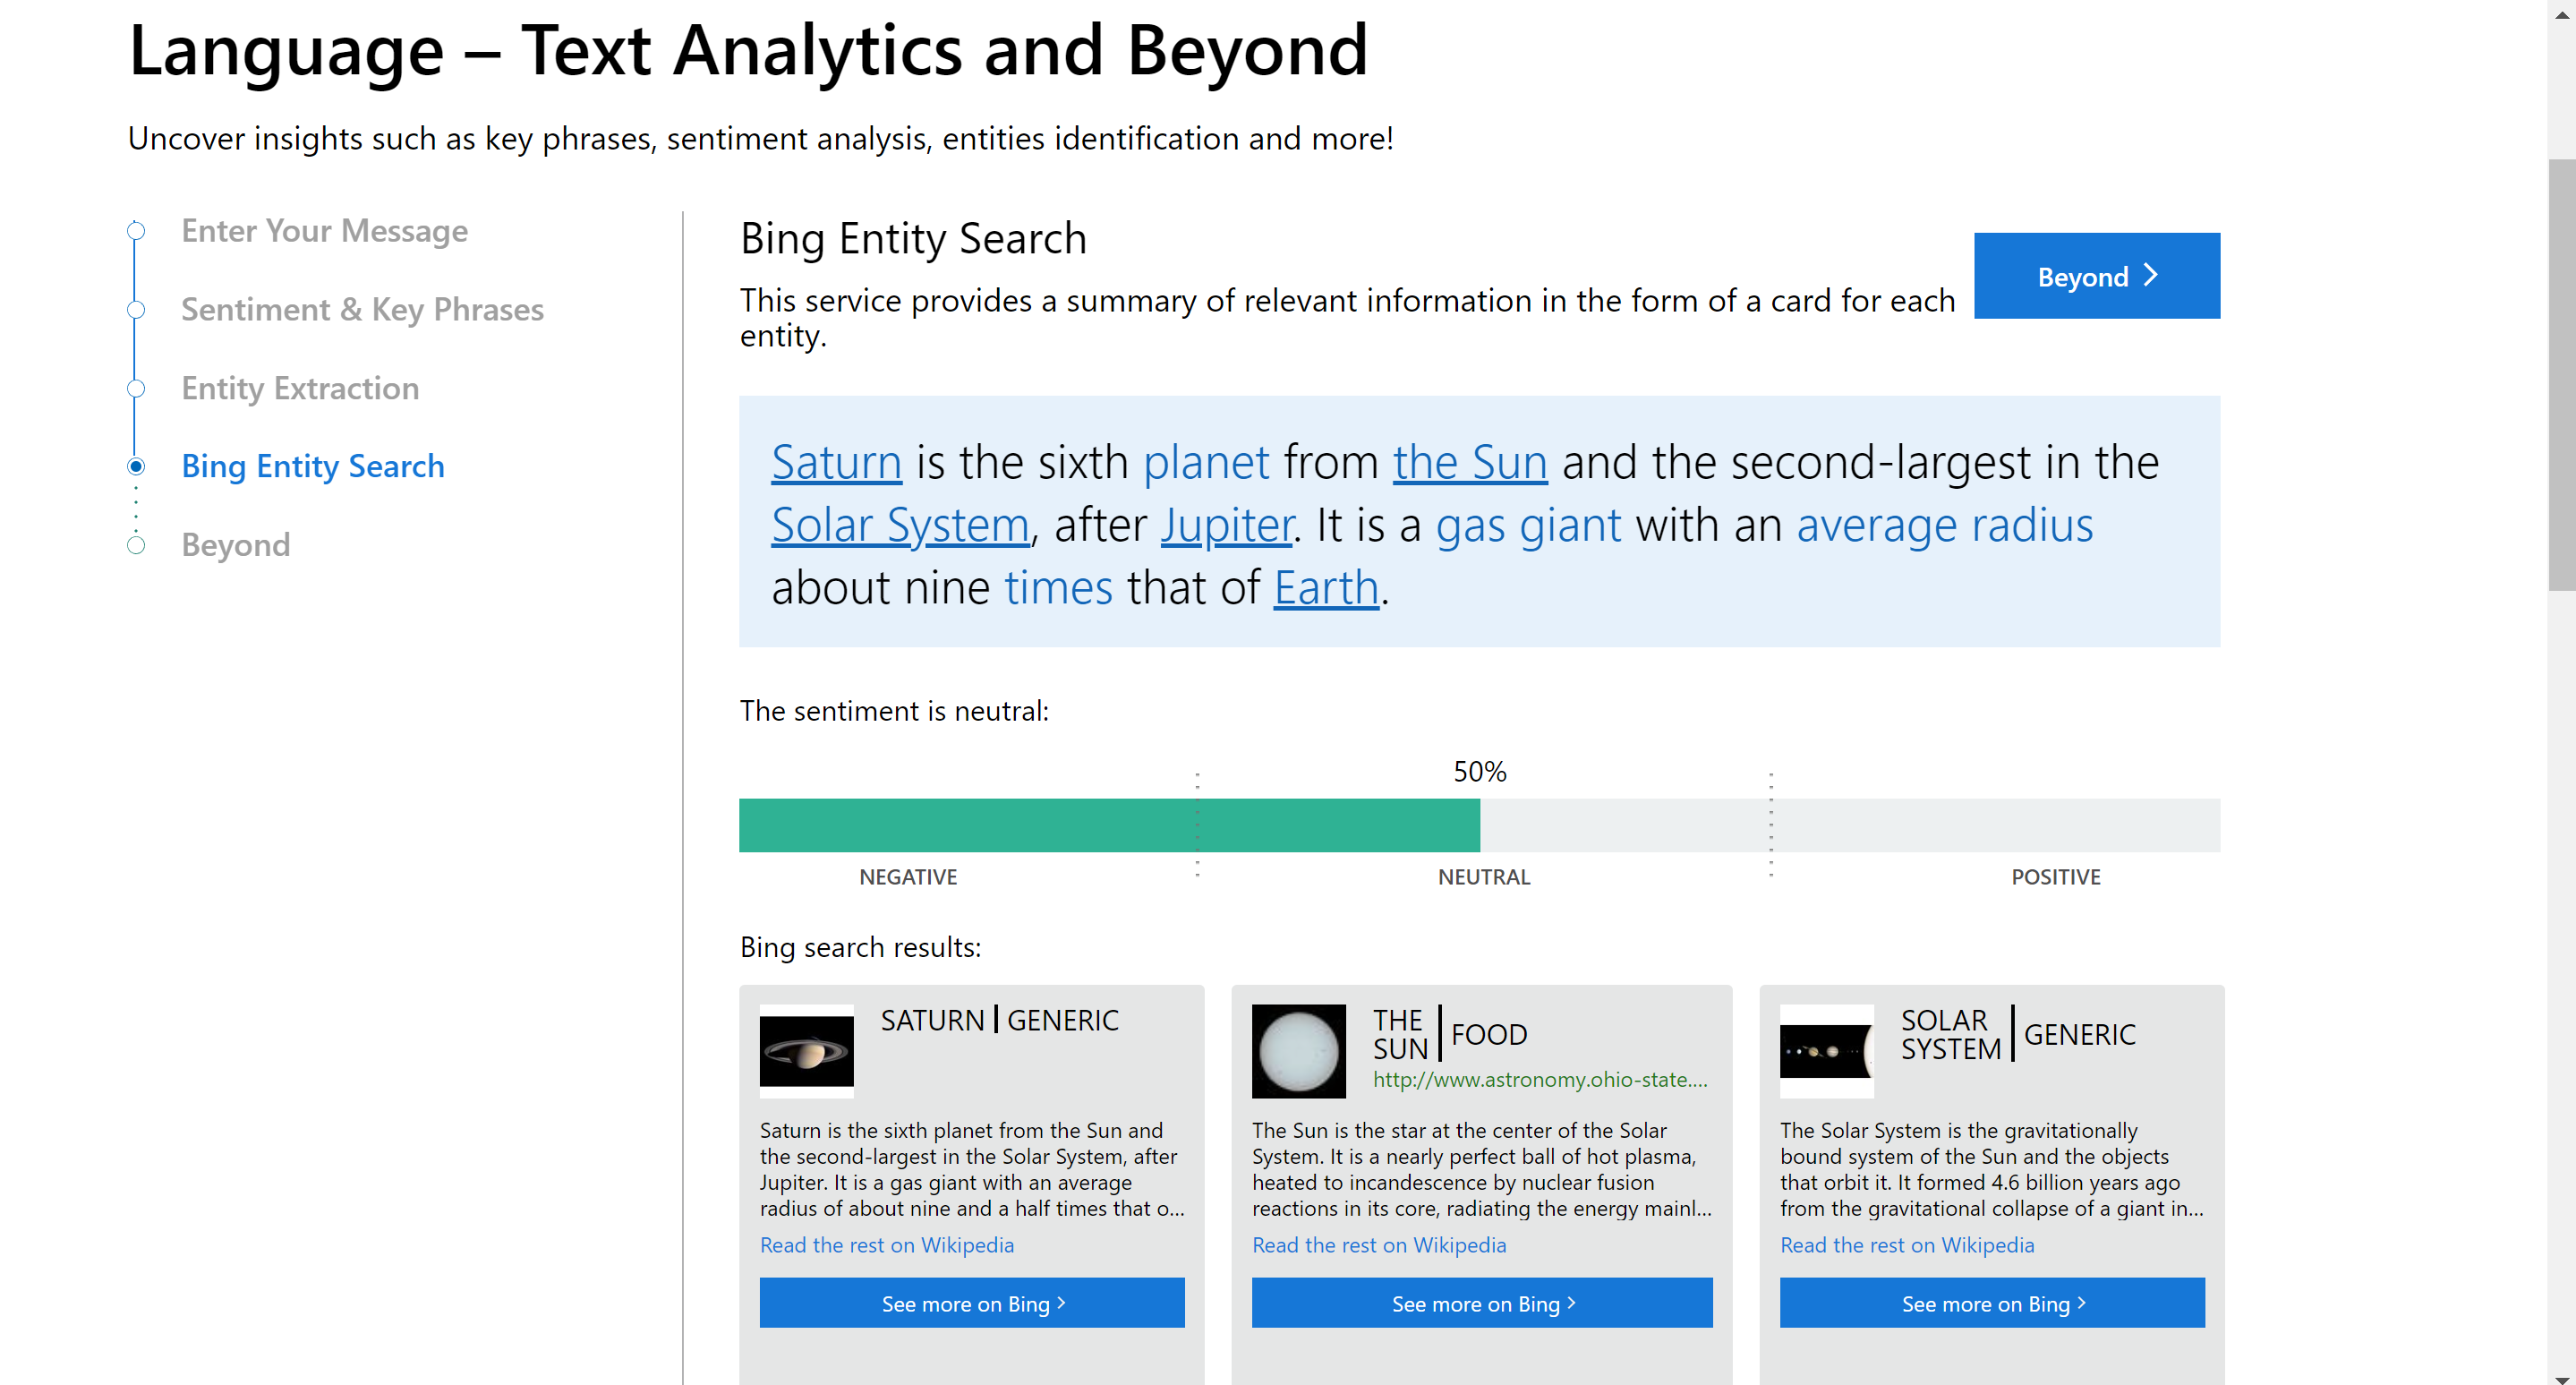
\includegraphics[width=150mm]{figs/msDemo.png}
    \caption{Servicii Microsoft AI}
	\label{fig:msDemo}
\end{figure}
\subsection{Google Trends}
{\noindent Acest serviciu are următoarele funcționalități:}
\begin{itemize}
    \setlength\itemsep{0.5em}
    \item Evoluția unui cuvânt sau a unei expresii într-o perioada de timp, într-o anumită regiune, dintr-o anumită categorie, căutare în mai multe formate
    \item Rezultatele sunt vizuale, afișate pe line chart-uri și hărți
    \item Sugestii de subiecte conexe și căutări similare
    \item Căutări populare zilnice și în timp real
    \item Căutările anului, pe categorii (Oameni, Emisiuni TV, Rețete, Simptome, etc.)
\end{itemize}
\begin{figure}[H]
	\centering
	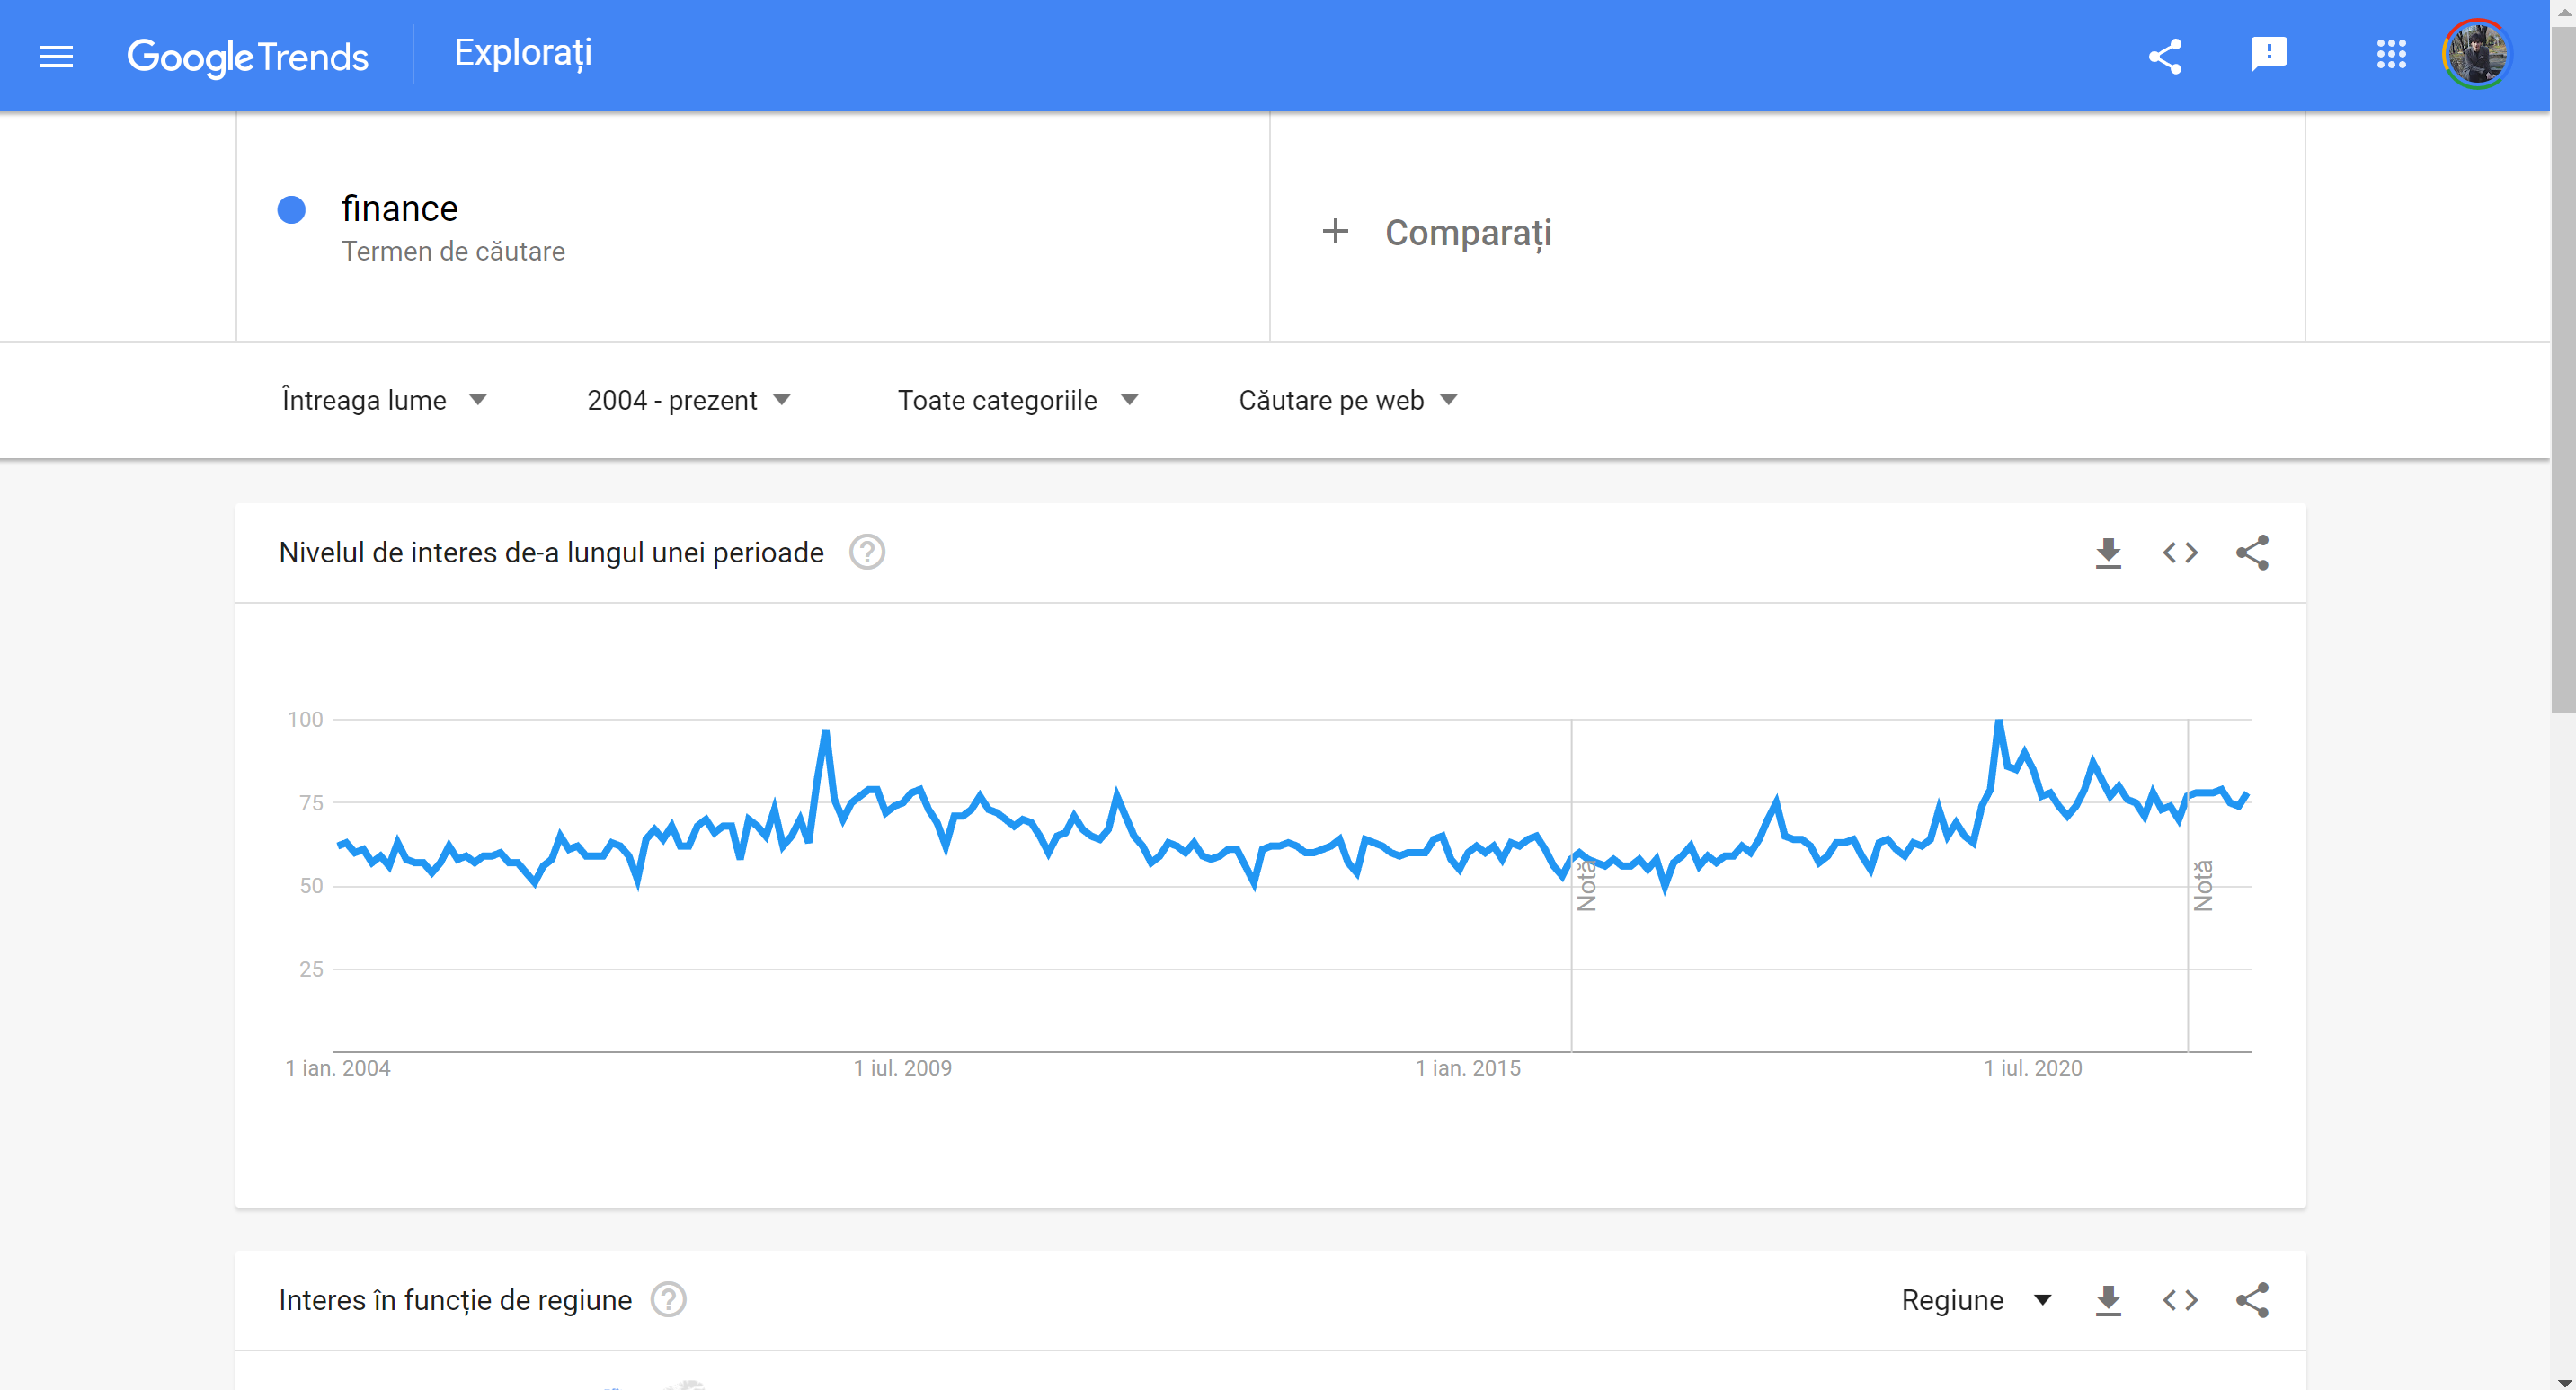
\includegraphics[width=150mm]{figs/googleTrends.png}
    \caption{Servicii Google Trends}
	\label{fig:googleTrends}
\end{figure}



\begin{table}[H]
	\caption{Comparație între aplicația prezentată și ale servicii existente}
	\centering                          % tabel centrat 
	\begin{tabular}{|c|c|c|c|c|c|}          % 4 coloane centrate 
		\hline
		 & IBM & Microsoft AI & Google Search & Google Trends & Aplicație\\ [2ex]   % inserare tabel
		%heading
		\hline                              % linie orizontal simpla
		Serviciu gratuit & NU & NU & NU & DA & DA \\[2ex]               % corpul tabelului 
		Sumarizare & NU & NU & NU & NU & DA \\ [2ex]
        Extracție entități & DA & DA & DA & NU & DA \\ [2ex]
        Analiză sentiment financiar & DA & NU & NU & NU & DA \\[2ex]
        Analiză popularitate & NU & NU & NU & DA & DA \\[2ex]
		Salvare analiză în cont & NU & NU & NU & NU & DA \\[2ex]           % [1ex] adds vertical space
        UI ușor de înțeles și folosit & NU & NU & NU & DA & DA \\[2ex] 
        \hline                              
	\end{tabular}
	% titlul tabelului
	\label{tab:nonlin}                % eticheta folosita pentru referirea tabelului in text; referirea in text se va face cu \ref{table:nonlin}
\end{table}